% Created 2023-02-19 Sun 16:52
% Intended LaTeX compiler: pdflatex
\documentclass[11pt]{article}
\usepackage[utf8]{inputenc}
\usepackage[T1]{fontenc}
\usepackage{graphicx}
\usepackage{longtable}
\usepackage{wrapfig}
\usepackage{rotating}
\usepackage[normalem]{ulem}
\usepackage{amsmath}
\usepackage{amssymb}
\usepackage{capt-of}
\usepackage{hyperref}
\graphicspath{{../../books/}}
% TIPS
% \substack{a\\b} for multiple lines text





% pdfplots will load xolor automatically without option
\usepackage[dvipsnames]{xcolor}

\usepackage{forest}
% two-line text in node by [two \\ lines]
% \begin{forest} qtree, [..] \end{forest}
\forestset{
  qtree/.style={
    baseline,
    for tree={
      parent anchor=south,
      child anchor=north,
      align=center,
      inner sep=1pt,
    }}}
%\usepackage{flexisym}
% load order of mathtools and mathabx, otherwise conflict overbrace

\usepackage{mathtools}
%\usepackage{fourier}
\usepackage{pgfplots}
\usepackage{amsthm, mathabx,  amsmath, commath}
\usepackage{amsfonts}

\usepackage{empheq}
\usepackage{tikz}
\usetikzlibrary{arrows.meta}
\usepackage[most]{tcolorbox}

\newtheorem{theorem}{Theorem}[section]
\newtheorem{definition}{Definition}[section]
\newtheorem{corollary}{Corollary}[section]
\newtheorem{example}{Example}[section]
\newtheorem{lemma}{Lemma}[section]
\newtheorem{proposition}{Proposition}[section]

\newcommand{\bl}[1] {\boldsymbol{#1}}
\newcommand{\Wt}[1] {\stackrel{\sim}{\smash{#1}\rule{0pt}{1.1ex}}}
\newcommand{\wt}[1] {\widetilde{#1}}


%For boxed texts in align, use Aboxed{}
%otherwise use boxed{}

\DeclareMathSymbol{\widehatsym}{\mathord}{largesymbols}{"62}
\newcommand\lowerwidehatsym{%
  \text{\smash{\raisebox{-1.3ex}{%
    $\widehatsym$}}}}
\newcommand\fixwidehat[1]{%
  \mathchoice
    {\accentset{\displaystyle\lowerwidehatsym}{#1}}
    {\accentset{\textstyle\lowerwidehatsym}{#1}}
    {\accentset{\scriptstyle\lowerwidehatsym}{#1}}
    {\accentset{\scriptscriptstyle\lowerwidehatsym}{#1}}
}

\usepackage{graphicx}
    
% text on arrow for xRightarrow
\makeatletter
%\newcommand{\xRightarrow}[2][]{\ext@arrow 0359\Rightarrowfill@{#1}{#2}}
\makeatother


\def \bx {\boldsymbol{x}}
\def \ba {\boldsymbol{a}}
\def \bI {\boldsymbol{I}}
\def \bt {\boldsymbol{t}}
\def \bb {\boldsymbol{b}}
\def \bA {\boldsymbol{A}}
\def \bX {\boldsymbol{X}}
\def \bu {\boldsymbol{u}}
\def \bS {\boldsymbol{S}}
\def \bZ {\boldsymbol{Z}}
\def \bz {\boldsymbol{z}}
\def \by {\boldsymbol{y}}
\def \bw {\boldsymbol{w}}
\def \bT {\boldsymbol{T}}
\def \bS {\boldsymbol{S}}
\def \bm {\boldsymbol{m}}
\def \bW {\boldsymbol{W}}
\def \bY {\boldsymbol{Y}}
\def \bH {\boldsymbol{H}}
\def \blambda {\boldsymbol{\lambda}}
\def \bPhi {\boldsymbol{\Phi}}
\def \btheta {\boldsymbol{\theta}}
\def \bmu {\boldsymbol{\mu}}
\def \bphi {\boldsymbol{\phi}}
\def \bSigma {\boldsymbol{\Sigma}}
\def \lb {\left\{}
\def \rb {\right\}}
\def \caln {\mathcal{N}}
\def \dissum {\displaystyle\Sigma}
\def \dispro {\displaystyle\prod}
\def \E {\mathbb{E}}
\def \Q {\mathbb{Q}}
\def \V {\mathbb{V}}
\def \R {\mathbb{R}}
\def \calq {\mathcal{Q}}
\def \calg {\mathcal{G}}
\def \caln {\mathcal{N}}
\def \calr {\mathcal{R}}
\def \calm {\mathcal{M}}
\def \calc {\mathcal{C}}
\def \bcup {\bigcup}

\usepackage{minted}
\setminted{fontsize=\footnotesize,baselinestretch=1}
\makeindex
\let\OldTexttt\texttt
\renewcommand{\texttt}[1]{\OldTexttt{\color{MidnightBlue} #1}}
\author{Bjarne Stroustrup}
\date{\today}
\title{A Tour Of C++}
\hypersetup{
 pdfauthor={Bjarne Stroustrup},
 pdftitle={A Tour Of C++},
 pdfkeywords={},
 pdfsubject={},
 pdfcreator={Emacs 28.0.92 (Org mode 9.6)}, 
 pdflang={English}}
\begin{document}

\maketitle
\tableofcontents

\section{The Basics}
\label{sec:orgbf5c049}
\subsection{Introduction}
\label{sec:orgabfe126}
The operator \texttt{<<} (``put to'') writes its second argument onto its first

A function declaration gives the name of the function, the type of the value returned (if any),
and the number and types of the arguments that must be supplied in a call

If two functions are defined with the same name, but with different argument types, the compiler
will choose the most appropriate function to invoke for each call.

Defining multiple functions with the same name is known as function \textbf{overloading} and is one of the
essential parts of generic programming
\subsection{Types, Variables and Arithemtic}
\label{sec:org4e19f02}
A \textbf{declaration} is a statement that introduces an entity into the program. It specifies a type for
the entity:
\begin{itemize}
\item A \textbf{type} defines a set of possible values and a set of operations (for an object)
\item An \textbf{object} is some memory that holds a value of some type.
\item A \textbf{value} is a set of bits interpreted according to a type.
\item A \textbf{variable} is a named object.
\end{itemize}


Unfortunately, conversions that lose information, \textbf{narrowing conversions}, such as \texttt{double} to \texttt{int}
and \texttt{int} to \texttt{char}, are allowed and implicitly applied when you use \texttt{=} (but not when you use \texttt{\{\}})

When defining a variable, you don’t need to state its type explicitly when it can be deduced
from the initializer:
\begin{minted}[]{c++}
    auto b = true;    // a bool
    auto ch = 'x';    // a char
    auto i = 123;     // an int
    auto d = 1.2;     // a double
    auto z = sqrt(y); // z has the type of whatever
                      // sqrt(y) returns 
    auto bb {true};   //bb is a bool
\end{minted}

With \texttt{auto}, we tend to use the \texttt{=} because there is no potentially troublesome type conversion
involved, but if you prefer to use \texttt{\{\}} initialization consistently, you can do that instead.
\subsection{Scope and Lifetime}
\label{sec:orgea10fce}
\begin{itemize}
\item \textbf{Local scope}: A name declared in a function or lambda is called a local name.
Its scope extends from its point of declaration to the end of the block in which its
declaration occurs. A \textbf{block} is delimited by a \texttt{\{ \}} pair. Function argument names are
considered local names.
\item \textbf{Class scope}: A name is called a \textbf{member name} (or a \textbf{class member name}) if it is defined in a
class , outside any function , lambda, or enum class. Its scope extends from the opening \texttt{\{} of
its enclosing declaration to the end of that declaration.
\item \textbf{Namespace scope}: A name is called a \textbf{namespace member name} if it is defined in a namespace
outside any function, lambda, class, or enum class. Its scope extends from the point of
declaration to the end of its namespace.

\begin{minted}[]{c++}
vector<int> vec; // vec is global 
struct Record {  
    string name; // name is a member of Record 
// ...
};
void fct(int arg) { // fct is global (a global function)
                    // arg is local (an integer argument)
    string motto {"Who dares wins"}; // motto is local
    auto p = new Record{"Hume"};
    // p points to an unnamed Record (created by new)
    // ...
}
\end{minted}
\end{itemize}
\subsection{Constants}
\label{sec:orgcb942ff}
C++ supports two notions of immutability:
\begin{itemize}
\item \texttt{const}: meaning roughly ``I promise not to change this value.'' This is used primarily to
specify interfaces so that data can be passed to functions using pointers and references without
fear of it being modified. The compiler enforces the promise made by \texttt{const}. The value of a \texttt{const} can
be calculated at run time.
\item \texttt{constexpr}: meaning roughly ``to be evaluated at compile time.'' This is used primarily to
specify constants, to allow placement of data in read-only memory (where it is unlikely to
be corrupted), and for performance. The value of a \texttt{constexpr} must be calculated by the
compiler.
\end{itemize}


For example
\begin{minted}[]{c++}
constexpr int dmv = 17;           // dmv is a named constant
int var = 17;                     // var is not a constant
const double sqv = sqrt(var);     // sqv is a named constant,
                                  // possibly computed at run time
double sum(const vector<double>&);// sum will not modify
                                  // its argument
vector<double> v {1.2, 3.4, 4.5}; // v is not a constant
const double s1 = sum(v);         // OK: sum(v) is evaluated at
                                  // run time
constexpr double s2 = sum(v);     // error: sum(v) is not a
                                  // constant expression
\end{minted}

For a function to be usable in a \textbf{constant expression}, that is, in an expression that will be
evaluated by the compiler, it must be defined \texttt{constexpr}. For example:
\begin{minted}[]{c++}
constexpr double square(double x) { return x∗x; }
constexpr double max1 = 1.4∗square(17);
// OK 1.4*square(17) is a constant expression
constexpr double max2 = 1.4∗square(var);
// error: var is not a constant expression 
const double max3 = 1.4∗square(var);
// OK, may be evaluated at run time
\end{minted}

A \texttt{constexpr} function can be used for non-constant arguments, but when that is done the result is
not a constant expression. We allow a \texttt{constexpr} function to be called with
non-constant-expression arguments in contexts that do not require constant expressions. That
way, we don’t have to define essentially the same function twice: once for constant expressions
and once for variables.

To be \texttt{constexpr}, a function must be rather simple and cannot have side effects and can only use
information passed to it as arguments. In particular, it cannot modify non-local variables, but
it can have loops and use its own local variables. For example:
\begin{minted}[]{c++}
constexpr double nth(double x, int n) // assume 0<=n {
{
    double res = 1;
    int i = 0;
    while (i<n) {
        res*=x;
        ++i;
    }
    return res;
}
\end{minted}
\subsection{Pointers, Arrays, and References}
\label{sec:org671e386}
\begin{minted}[]{c++}
char* p = &v[3];
char x = *p;
\end{minted}
in an expression, prefix unary \texttt{*} means ``contents of'' and prefix unary \texttt{\&} means ``address of''

If we didn’t want to copy the values from \texttt{v} into the variable \texttt{x}, but rather just have \texttt{x} refer to
an element, we could write:
\begin{minted}[]{c++}
void increment() {
    int v[] = {0,1,2,3,4,5,6,7,8,9};
    for (auto& x : v) // add 1 to each x in v
        ++x;
    // ...
}
\end{minted}

In a declaration, the unary suffix \texttt{\&} means ``reference to.'' A reference is similar to a
pointer, except that you don't need to use a prefix \texttt{*} to access the value referred to by the
reference. Also, a reference cannot be made to refer to a different object after its
initialization.

References are particularly useful for specifying function arguments. For example:
\begin{minted}[]{c++}
void sort(vector<double>& v); // sort v
                              // v is a vector of doubles
\end{minted}
By using a reference, we ensure that for a call \texttt{sort(vec)}, we do not copy \texttt{vec} and that it really
is \texttt{vec} that is sorted and not a copy of it.

When used in declarations, operators (such as \texttt{\&}, \texttt{*}, and \texttt{[]}) are called declarator operators:
\begin{minted}[]{c++}
T a[n] // T[n]: a is an array of n Ts
T∗ p   // T*: p is a pointer to T
T& r   // T&: r is a reference to T
T f(A) // T(A): f is a function taking an argument of type A
       // returning a result of type T
\end{minted}

We try to ensure that a pointer always points to an object so that dereferencing it is valid.
When we don't have an object to point to or if we need to represent the notion of ``no object
available'' (e.g., for an end of a list), we give the pointer the value \texttt{nullptr} (``the null
pointer''). There is only one \texttt{nullptr} shared by all pointer types:
\begin{minted}[]{c++}
double∗ pd = nullptr;
Link<Record>∗ lst = nullptr; // pointer to a Link to a Record
int x = nullptr; // error: nullptr is a pointer not an integer
\end{minted}
\subsection{Tests}
\label{sec:orgc8b5f6f}
\subsection{Mapping to Hardware}
\label{sec:org1a423bd}
An assignment of a built-in type is a simple machine copy operation.

A reference and a pointer both refer/point to an object and both are represented in memory as a
machine address. However, the language rules for using them differ. Assignment to a reference
does not change what the reference refers to but assigns to the referenced object:
\begin{minted}[]{c++}
int x = 2;
int y = 3;
int& r = x; // r refers to x
int& r2 = y; // now r2 refers to y
r = r2; // read through r2, write through r: x becomes 3
\end{minted}
\begin{figure}[htbp]
\centering
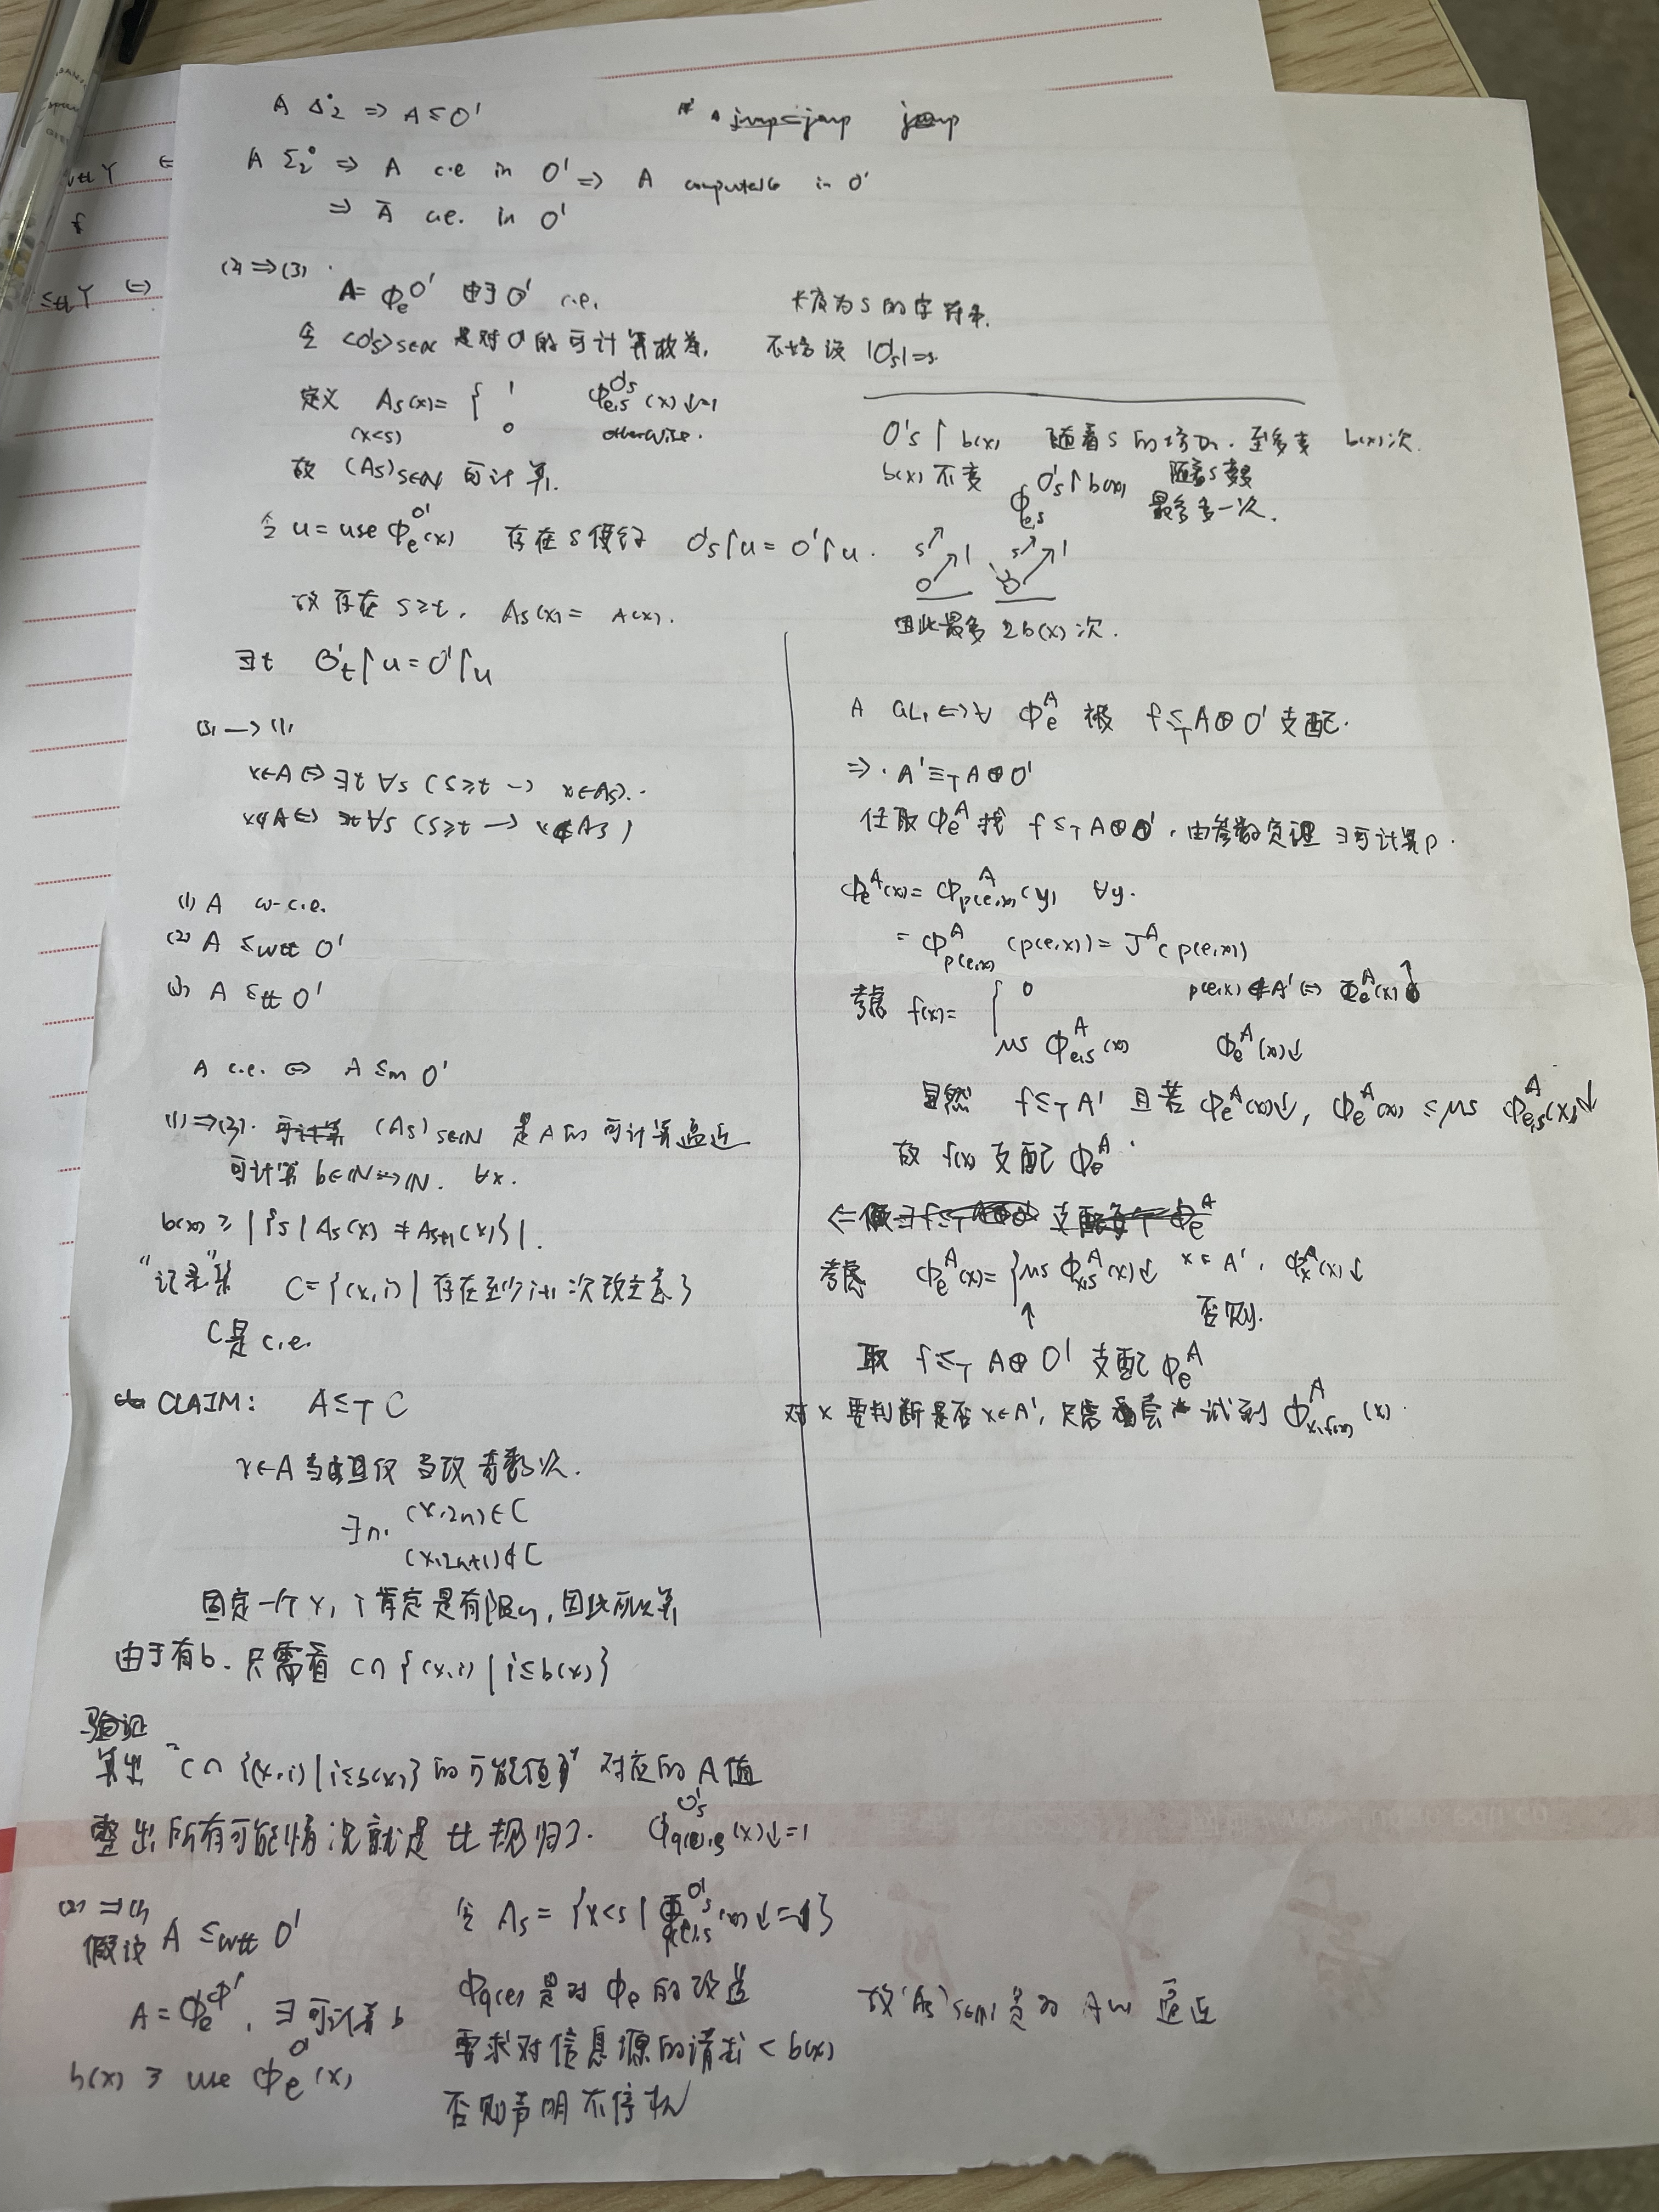
\includegraphics[width=.6\textwidth]{../images/ATourOfC++/1.png}
\label{}
\end{figure}
\section{User-Defined Types}
\label{sec:orgcdd071f}
\subsection{Introduction}
\label{sec:org80ab8fb}
Types built out of other types using C++’s abstraction mechanisms are called \textbf{user-defined types}.
They are referred to as \textbf{classes} and \textbf{enumerations}.
\subsection{Structures}
\label{sec:org72ba6fc}
The \texttt{new} operator allocates memory from an area called the \textbf{free store} (also known as \textbf{dynamic
memory} and \textbf{heap}). Objects allocated on the free store are independent of the scope from which
they are created and ``live'' until they are destroyed using the \texttt{delete} operator
\subsection{Classes}
\label{sec:orgdae2530}
The language mechanism for that is called a \textbf{class}. A class has a set of \textbf{members}, which can be
data, function, or type members. The interface is defined by the \texttt{public} members of a class, and
\texttt{private} members are accessible only through that interface.
\label{Vector}
\begin{minted}[]{c++}
class Vector {
    public:
        Vector(int s) :elem{new double[s]}, sz{s} { }
        double& operator[](int i) { return elem[i]; }
        int size() { return sz; }
    private:
        double* elem; // pointer to the elements
        int sz; // the number of elements
};
\end{minted}

\texttt{Vector(int)} defines how objects of type \texttt{Vector} are constructed. The constructor initializes the
\texttt{Vector} members using a member initializer list:
\begin{minted}[]{c++}
:elem{new double[s]}, sz{s}
\end{minted}
That is, we first initialize \texttt{elem} with a pointer to \texttt{s} elements of type \texttt{double} obtained from the
free store. Then, we initialize \texttt{sz} to \texttt{s}

Access to elements is provided by a subscript function, called \texttt{operator[]}. It returns a
reference to the appropriate element (a \texttt{double\&} allowing both reading and writing)

There is no \uline{fundamental} difference between a \texttt{struct} and a \texttt{class}; a \texttt{struct} is simply a class with
members \texttt{public} by default.
\subsection{Unions}
\label{sec:org0ca7b93}
A \texttt{union} is a \texttt{struct} in which all members are allocated at the same address so that the \texttt{union}
occupies only as much space as its largest member. Naturally, a \texttt{union} can hold a value for
only one member at a time.
\begin{minted}[]{c++}
union Value {
    Node* p;
    int i;
};
\end{minted}
The language doesn’t keep track of which kind of value is held by a union, so the programmer
must do that:
\begin{minted}[]{c++}
enum Type { ptr, num }; // a Type can hold values ptr and num

struct Entry {
    string name;
    Type t;
    Value v; // use v.p if t==ptr; use v.i if t==num
};

void f(Entry* pe) {
    if (pe->t == num)
        cout << pe->v.i;
    // ...
}
\end{minted}
Maintaining the correspondence between a \textbf{type field} (here, \texttt{t}) and the type held in a \texttt{union} is
error-prone.

The standard library type, \texttt{variant}, can be used to eliminate most direct uses of unions. A
\texttt{variant} stores a value of one of a set of alternative types.
\begin{minted}[]{c++}
struct Entry {
    string name;
    variant<Node∗,int> v;
};

void f(Entry∗ pe) {
if (holds_alternative<int>(pe−>v))
    // does *pe hold an int?
    cout << get<int>(pe−>v);
    // get the int
    // ...
} 
\end{minted}

For many uses, a \texttt{variant} is simpler and safer to use than a \texttt{union}
\subsection{Enumerations}
\label{sec:org187f8fe}
\begin{minted}[]{c++}
enum class Color { red, blue, green };
enum class Traffic_light { green, yellow, red };
Color col = Color::red;
Traffic_light light = Traffic_light::red;
\end{minted}

Note that enumerators (e.g., \texttt{red}) are in the scope of their \texttt{enum class}, so that they can be used
repeatedly in different \texttt{enum classes} without confusion. For example, \texttt{Color::red} is \texttt{Color} ’s \texttt{red}
which is different from \texttt{Traffic\_light::red}.

Enumerations are used to represent small sets of integer values. They are used to make code more
readable and less error-prone than it would have been had the symbolic (and mnemonic) enumerator
names not  been used.

The \texttt{class} after the \texttt{enum} specifies that an enumeration is strongly typed and that its
enumerators are scoped.
\begin{minted}[]{c++}
Color x = red; // error : which red?
Color y = Traffic_light::red;
// error: that red is not a Color
Color z = Color::red; // OK
\end{minted}

Similarly, we cannot implicitly mix \texttt{Color} and integer values:
\begin{minted}[]{c++}
int i = Color::red; // error: Color::red is not an int
Color c = 2; // initialization error: 2 is not a Color
\end{minted}

By default, an \texttt{enum class} has only assignment, initialization, and comparisons. However, an
enumeration is a user-defined type, so we can define operators for it:
\begin{minted}[]{c++}
Traffic_light& operator++(Traffic_light& t)
{ // prefix increment: ++ 
        switch (t) {
            case Traffic_light::green:
                return t=Traffic_light::yellow;
            case Traffic_light::yellow:
                return t=Traffic_light::red;
            case Traffic_light::red:
                return t=Traffic_light::green;
}
}
Traffic_light next = ++light;
// next becomes Traffic_light::green
\end{minted}

If you don’t want to explicitly qualify enumerator names and want enumerator values to be ints
(without the need for an explicit conversion), you can remove the \texttt{class} from \texttt{enum class} to get a
``plain'' \texttt{enum}. The enumerators from a ``plain'' \texttt{enum} are entered into the same scope as the
name of their enum and implicitly converts to their integer value

\begin{minted}[]{c++}
enum Color { red, green, blue };
int col = green;
\end{minted}
Here \texttt{col} gets the value 1. By default, the integer values of enumerators start with \texttt{0} and
increase by one for each additional enumerator.
\section{Modularity}
\label{sec:orgbe6a361}
\subsection{Introduction}
\label{sec:orgbe888da}
A \textbf{declaration} specifies all that’s needed to use a function or a type. For example:
\begin{minted}[]{c++}
double sqrt(double);
// the square root function takes a double and returns a double
class Vector {
    public:
        Vector(int s);
        double& operator[](int i); int size();
    private:
        double∗ elem; // elem points to an array of
                      // sz doubles int sz;
};        
\end{minted}

The key point here is that the function bodies, the function \textbf{definitions}, are ``elsewhere''

The definition of \texttt{sqrt()} will look like this:
\begin{minted}[]{c++}
double sqrt(double d) // definition of sqrt()
{
    // ... algorithm as found in math textbook ...
}
\end{minted}

For \texttt{vector}, we need to define
\begin{minted}[]{c++}
Vector::Vector(int s) // definition of the constructor
    :elem{new double[s]}, sz{s}
     // initialize members
{
}
double& Vector::operator[](int i) {
    // definition of subscripting
    return elem[i];
}
int Vector::size() {
    // definition of size()
    return sz;
}
\end{minted}
\subsection{Separate Compilation}
\label{sec:org3ec2af8}
C++ supports a notion of separate compilation where user code sees only declarations of the
types and functions used. The definitions of those types and functions are in separate source
files and are compiled separately.

This can be used to organize a program into a set of semi-independent code fragments. Such
separation can be used to minimize compilation times and to strictly enforce sepa- ration of
logically distinct parts of a program (thus minimizing the chance of errors). A library is often
a collection of separately compiled code fragments (e.g., functions).

Typically, we place the declarations that specify the interface to a module in a file with a
name indicating its intended use. Example:
\begin{minted}[]{c++}
// Vector.h:
class Vector {
    public:
        Vector(int s);
        double& operator[](int i); int size();
    private:
        double∗ elem;
        int sz;
};
\end{minted}

This declaration would be placed in a file \texttt{Vector.h}. Users then \textbf{include} that file, called a
\textbf{header file}, to access that interface. For example:
\begin{minted}[]{c++}
// user.cpp:
#include "Vector.h" // get Vector’s interface
#include <cmath> // get the standard-library
                 // math function interface including sqrt()
double sqrt_sum(Vector& v)
{
    double sum = 0;
    for (int i=0; i!=v.size(); ++i)
        sum+=std::sqrt(v[i]);
    return sum;
}
\end{minted}

To help the compiler ensure consistency, the \texttt{.cpp} file providing the implementation of \texttt{Vector}
will also include the .h file providing its interface:
\begin{minted}[]{c++}
// Vector.cpp:
#include "Vector.h" // get Vector’s interface
                
Vector::Vector(int s)
    :elem{new double[s]}, sz{s}
{    
}
double& Vector::operator[](int i)
{
    return elem[i];
}
int Vector::size()
{
    return sz;
}
\end{minted}

The code in \texttt{user.cpp} and \texttt{Vector.cpp} shares the \texttt{Vector} interface information presented in
\texttt{Vector.h}, but the two files are otherwise independent and can be separately compiled.

A \texttt{.cpp} file that is compiled by itself (including the h files it \texttt{\#includes}) is called a
\textbf{translation unit}. A program can consist of many thousand translation units.
\subsection{Modules (C++20)}
\label{sec:orgc85bd66}
The use of \texttt{\#includes} is a very old, error-prone, and rather expensive way of composing programs
out of parts. If you \texttt{\#include header.h} in 101 translation units, the text of \texttt{header.h} will be
processed by the compiler 101 times. If you \texttt{\#include header1.h} before \texttt{header2.h} the declarations
and macros in \texttt{header1.h} might affect the meaning of the code in \texttt{header2.h}. If instead you
\texttt{\#include header2.h} before \texttt{header1.h}, it is \texttt{header2.h} that might affect the code in \texttt{header1.h}.
Obviously, this is not ideal, and in fact it has been a major source of cost and bugs since 1972
when this mechanism was first introduced into C.

Consider how to express the \texttt{Vector} and \texttt{sqrt\_sum()} example from §3.2 using \texttt{modules}:
\begin{minted}[]{c++}
// file Vector.cpp:
module; // this compilation will define a module
// ... here we put stuff that Vector might
// need for its implementation ...
export module Vector; // defining the module called "Vector"

export class Vector {
    public:
        Vector(int s);
        double& operator[](int i); int size();
    private:
        double∗ elem; // elem points to an array of sz doubles
        int sz;
};

Vector::Vector(int s)
:elem{new double[s]}, sz{s}
{
}

double& Vector::operator[](int i)
{
return elem[i];
}

int Vector::size()
{
return sz;
}

export int size(const Vector& v) { return v.size(); }
\end{minted}
This defines a module called \texttt{Vector}, which exports the class Vector, all its member functions,
and the non-member function \texttt{size()}

The way we use this module is to \texttt{import} it where we need it. For example:.
\begin{minted}[]{c++}
// file user.cpp:
// 
import Vector; // get Vector’s interface
#include <cmath>

double sqrt_sum(Vector& v)
{
    double sum = 0;
    for (int i=0; i!=v.size(); ++i)
        sum+=std::sqrt(v[i]);
    return sum;
}
\end{minted}

The differences between headers and modules are not just syntactic.
• A module is compiled once only (rather than in each translation unit in which it is used).
• Two modules can be \texttt{imported} in either order without changing their meaning.
• If you import something into a module, users of your module do not implicitly gain access
   to (and are not bothered by) what you imported: \texttt{import} is not transitive.
\subsection{Namespaces}
\label{sec:org1176f78}
C++ offers \textbf{namespaces} as a mechanism for expressing that some declarations belong together and
that their names shouldn’t clash with other names

\begin{minted}[]{c++}
namespace My_code {
    class complex {
        // ...
    };
    complex sqrt(complex);
    // ...
    int main();
}

int My_code::main()
{
    complex z {1,2};
    auto z2 = sqrt(z);
    std::cout << '{' << z2.real() << ',' << z2.imag() << "}\n";
    // ...
}

int main()
{
    return My_code::main();
}
\end{minted}
By putting my code into the namespace \texttt{My\_code}, I make sure that my names do not conflict
with the standard-library names in namespace \texttt{std}

If repeatedly qualifying a name becomes tedious or distracting, we can bring the name into a
scope with a \texttt{using}-declaration:
\begin{minted}[]{c++}
void my_code(vector<int>& x, vector<int>& y)
{
    using std::swap; // ...
    swap(x,y);
    other::swap(x,y); // ...
}
\end{minted}

To gain access to all names in the standard-library namespace, we can use a \texttt{using}-directive:
\begin{minted}[]{c++}
using namespace std;
\end{minted}
\subsection{Error Handling}
\label{sec:orga0a5d01}
\subsubsection{Exceptions}
\label{sec:orgdc13033}
Consider again the \texttt{Vector} example.

Assuming that out-of-range access is a kind of error that we want to recover from, the solution
is for the \texttt{Vector} implementer to detect the attempted out-of-range access and tell the user
about it. The user can then take appropriate action. For example, \texttt{Vector::operator[]()} can
detect an attempted out-of-range access and throw an \texttt{out\_of\_range} exception:
\begin{minted}[]{c++}
double& Vector::operator[](int i)
{
    if (i<0 || size()<=i)
        throw out_of_range{"Vector::operator[]"};
    return elem[i];
}
\end{minted}
The \texttt{throw} transfers control to a handler for exceptions of type \texttt{out\_of\_range} in some function that
directly or indirectly called \texttt{Vector::operator[]()}. To do that, the implementation will \textbf{unwind}
the function call stack as needed to get back the context of that caller. That is, the exception
handling mechanism will exit scopes and functions as needed to get back to a caller that has
expressed interest in handling that kind of exception, invoking destructors (§4.2.2) along the
way as needed. For example:

\begin{minted}[]{c++}
void f(Vector& v) {
// ...
    try { // exceptions here are handled by
          // the handler defined below
        v[v.size()] = 7; // try to access beyond the end of v
    }
    catch (out_of_range& err) {
    // ... handle range error ...
        cerr << err.what() << '\n';
    }
    // ...
}
\end{minted}

We put code for which we are interested in handling exceptions into a \texttt{try}-block. The attempted
assignment to \texttt{v[v.size()]} will fail. Therefore, the \texttt{catch}-clause providing a handler for
exceptions of type \texttt{out\_of\_range} will be entered. The \texttt{out\_of\_range} type is defined in the standard
library (in \texttt{<stdexcept>}) and is in fact used by some standard-library container access
functions.

The main technique for making error handling simple and systematic (called \textbf{Resource Acquisition
Is Initialization}; RAII) is explained in §4.2.2. The basic idea behind RAII is for a constructor
to acquire all resources necessary for a class to operate and have the destructor release all
resources, thus making resource release guaranteed and implicit.

A function that should never throw an exception can be declared \texttt{noexcept}. For example:
\begin{minted}[]{c++}
void user(int sz) noexcept {
    Vector v(sz);
    iota(&v[0],&v[sz],1); // fill v with 1,2,3,4...
    // ...
}
\end{minted}
\subsubsection{Invariants}
\label{sec:org0bacd06}
The use of exceptions to signal out-of-range access is an example of a function checking its
argument and refusing to act because a basic assumption, a \textbf{precondition}, didn’t hold
\begin{minted}[]{c++}
Vector::Vector(int s)
{
    if (s<0)
        throw length_error{"Vector constructor: negative size"};
    elem = new double[s];
    sz = s;
}
\end{minted}

If operator \texttt{new} can’t find memory to allocate, it throws a \texttt{std::bad\_alloc}.
\begin{minted}[]{c++}
void test()
{
    try {
        Vector v(−27);
    }
    catch (std::length_error& err) {
// handle negative size
    }
    catch (std::bad_alloc& err) {
// handle memory exhaustion
    }
}
\end{minted}

Often, a function has no way of completing its assigned task after an exception is thrown. Then,
‘‘handling’’ an exception means doing some minimal local cleanup and rethrowing the exception.
\begin{minted}[]{c++}
void test()
{
    try {
        Vector v(−27);
    }
    catch (std::length_error&) {
        // do something and rethrow
        cerr << "test failed: length error\n";
        throw; // rethrow
    }
    catch (std::bad_alloc&) {
        // Ouch! this program is not designed to handle memory exhaustion
        std::terminate(); // terminate the program
    }
}
\end{minted}
\subsubsection{Error-Handling Alternatives}
\label{sec:orgff12884}
Throwing an exception is not the only way of reporting an error that cannot be handled locally.
A function can indicate that it cannot perform its allotted task by:
• throwing an exception
• somehow return a value indicating failure
• terminating the program (by invoking a function like \texttt{terminate()}, \texttt{exit()}, or \texttt{abort())}.


One way to ensure termination is to add \texttt{noexcept} to a function so that a \texttt{throw} from anywhere in
the function’s implementation will turn into a \texttt{terminate()}.
\subsubsection{Contracts}
\label{sec:org40e7578}
The standard library offers the debug macro, \texttt{assert()}, to assert that a condition must hold at
run time. For example:
\begin{minted}[]{c++}
void f(const char∗ p)
{
    assert(p!=nullptr);
    // p must not be the nullptr
}
\end{minted}
If the condition of an \texttt{assert()} fails in ``debug mode'', the program terminates
\subsubsection{Static Assertions}
\label{sec:org72a6a25}
Exceptions report errors found at run time. If an error can be found at compile time, it is
usually preferable to do so.

The \texttt{static\_assert} mechanism can be used for anything that can be expressed in terms of constant
expressions
\begin{minted}[]{c++}
constexpr double C = 299792.458; // km/s
void f(double speed)
{
    constexpr double local_max = 160.0/(60∗60); // 160 km/h == 160.0/(60*60) km/s
    static_assert(speed<C,"can't go that fast"); // error: speed must be a constant
    static_assert(local_max<C,"can't go that fast"); // OK
    // ...
}
\end{minted}

In general, \texttt{static\_assert(A,S)} prints \texttt{S} as a compiler error message if \texttt{A} is not \texttt{true}. If you
don’t want a specific message printed, leave out the \texttt{S} and the compiler will supply a default message:

\section{Classes}
\label{sec:org9244e6f}
\subsection{Introduction}
\label{sec:org490e5c9}
\subsection{Concrete Types}
\label{sec:orgf24f83e}
The basic idea of \textbf{concrete classes} is that they behave ‘‘just like built-in types.’’
\subsubsection{An Arithmetic Type}
\label{sec:org1b14da4}
\label{complex}
\begin{minted}[]{c++}
class complex {
    double re, im; // representation: two doubles
    public:
        // construct complex from two scalars
        complex(double r, double i) :re{r}, im{i} {}
        // construct complex from one scalar
        complex(double r) :re{r}, im{0} {}
        // default complex: {0,0}
        complex() :re{0}, im{0} {}
        
        double real() const { return re; }
        void real(double d) { re=d; }
        double imag() const { return im; }
        void imag(double d) { im=d; }
        
        complex& operator+=(complex z) {
            re+=z.re; // add to re and im im+=z.im;
            return *this; // and return the result
        }
        complex& operator-=(complex z) {
            re-=z.re;
            im-=z.im;
            return *this;
        }
        complex& operator*=(complex); // defined out-of-class somewhere
        complex& operator/=(complex); // defined out-of-class somewhere
};
\end{minted}

\texttt{complex} must be efficient or it will remain unused. This implies that simple operations must be
inlined. That is, simple operations (such as constructors, \texttt{+=}, and \texttt{imag()}) must be implemented
without function calls in the generated machine code. \textbf{Functions defined in a class are inlined
by default}. It is possible to explicitly request inlining by preceding a function declaration
with the keyword \texttt{inline}

A constructor that can be invoked without an argument is called a \textbf{default constructor}.

The \texttt{const} specifiers on the functions returning the real and imaginary parts indicate that these
functions do not modify the object for which they are called. A \texttt{const} member function can be
invoked for both \texttt{const} and non-\texttt{const} objects, but a non-\texttt{const} member function can only be
invoked for non-\texttt{const} objects. \href{https://stackoverflow.com/questions/3141087/what-is-meant-with-const-at-end-of-function-declaration}{stackexchange}

\begin{minted}[]{c++}
complex z = {1,0};
const complex cz {1,3};
z = cz; // OK: assigning to a non-const variable
cz = z; // error: complex::operator=() is a non-const member function double
x = z.real(); // OK: complex::real() is a const member function
\end{minted}

Many useful operations do not require direct access to the representation of complex, so they
can be defined separately from the class definition:
\begin{minted}[]{c++}
complex operator+(complex a, complex b) { return a+=b; }
complex operator−(complex a, complex b) { return a-=b; }
complex operator−(complex a) { return {−a.real(), −a.imag()}; }
complex operator∗(complex a, complex b) { return a*=b; }
complex operator/(complex a, complex b) { return a/=b; }
\end{minted}

The compiler converts operators involving complex numbers into appropriate function calls. For
example, \texttt{c!=b} means operator \texttt{!=(c,b)} and \texttt{1/a} means operator \texttt{/(complex\{1\},a)}.

User-defined operators (``overloaded operators'') should be used cautiously and conventionally.
The syntax is fixed by the language, so you can’t define a unary \texttt{/}. Also, it is not possible to
change the meaning of an operator for built-in types, so you can’t redefine \texttt{+} to subtract \texttt{ints}.
\subsubsection{A Container}
\label{sec:org0b3d16d}
A \textbf{container} is an object holding a collection of elements.

We need a mechanism to ensure that the memory allocated by the constructor is deallocated; that
mechanism is a \textbf{destructor}

\begin{minted}[]{c++}
class Vector { public:
        Vector(int s) :elem{new double[s]}, sz{s}
        // constructor: acquire resources
        {
            // initialize elements
            for (int i=0; i!=s; ++i)
                elem[i]=0;
        }
        // destructor: release resources
        ~Vector() { delete[] elem; }
        
        double& operator[](int i);
        int size() const;
        
    private:
        double* elem; // elem points to an array of sz doubles
        int sz;
};
\end{minted}

\texttt{Vector}'s constructor allocates some memory on the free store (also called the \textbf{heap} or \textbf{dynamic}
\textbf{store}) using the \texttt{new} operator. The destructor cleans up by freeing that memory using the
\texttt{delete[]} operator. Plain \texttt{delete} deletes an individual object, \texttt{delete[]} deletes an array.

The technique of acquiring resources in a constructor and releasing them in a destructor, known
as \textbf{Resource Acquisition Is Initialization} or \textbf{RAII}, allows us to eliminate ``naked \texttt{new}
operations'', that is, to avoid allocations in general code and keep them buried inside the
implementation of well-behaved abstractions.
\subsubsection{Initializing Containers}
\label{sec:org71b6d36}
\begin{itemize}
\item \textbf{Initializer-list constructor}: Initialize with a list of elements.
\item \texttt{push\_back()}: Add a new element at the end of (at the back of) the sequence.
\end{itemize}


\begin{minted}[]{c++}
class Vector {
    public:
        // initialize with a list of doubles
        Vector(std::initializer_list<double>); 
        // ...
        // add element at end, increasing the size by one 
        void push_back(double);
        // ...
};
\end{minted}

The \texttt{push\_back()} is useful for input of arbitrary numbers of elements
\begin{minted}[]{c++}
Vector read(istream& is) {
    Vector v;
    for (double d; is>>d; ) // read floating-point values into d
        v.push_back(d); // add d to v return v;
}
\end{minted}

The input loop is terminated by an end-of-file or a formatting error.

The way to provide Vector with a move constructor, so that returning a potentially huge amount
of data from read() is cheap
\begin{minted}[]{c++}
Vector v = read(cin); // no copy of Vector elements here
\end{minted}

The \texttt{std::initializer\_list} used to define the initializer-list constructor is a standard-library
type known to the compiler: when we use a \texttt{\{\}}-list, such as \texttt{\{1,2,3,4\}}, the compiler will create
an object of type \texttt{initializer\_list} to give to the program. So, we can write:
\begin{minted}[]{c++}
 // v1 has 5 elements Vector
Vector v1 = {1,2,3,4,5};
// v2 has 4 elements
v2 = {1.23, 3.45, 6.7, 8};
\end{minted}
\texttt{Vector}'s initializer-list constructor might be defined like this:
\begin{minted}[]{c++}
Vector::Vector(std::initializer_list<double> lst) // initialize with a list
    :elem{new double[lst.size()]}, sz{static_cast<int>(lst.size())}
{
    copy(lst.begin(),lst.end(),elem); // copy from lst into elem (§12.6)
}
\end{minted}

Unfortunately, the standard-library uses \texttt{unsigned} integers for sizes and subscripts, so I need
to use the ugly \texttt{static\_cast} to explicitly convert the size of the initializer list to an \texttt{int}

A \texttt{static\_cast} does not check the value it is converting; the programmer is trusted to use it
correctly.

Other casts are \texttt{reinterpret\_cast} for treating an object as simply a sequence of bytes and
\texttt{const\_cast} for ``casting away \texttt{const}.''
\subsection{Abstract Types}
\label{sec:orgbb11c2d}
an \textbf{abstract type} is a type that completely insulates a user from implementation details

First, we define the interface of a class \texttt{Container}, which we will design as a more abstract
version of our \texttt{Vector}:
\begin{minted}[]{c++}
class Container {
    public:
        // pure virtual function
        virtual double& operator[](int) = 0;
        // const member function (§4.2.1) 
        virtual int size() const = 0;
        // destructor (§4.2.2)
        virtual ~Container() {}
};
\end{minted}

The word \texttt{virtual} means ``may be redefined later in a class derived from this one'', and a function
declared \texttt{virtual} is called a \textbf{virtual function}.

A class derived from \texttt{Container} provides an implementation for the \texttt{Container} interface. The
curious \texttt{=0} syntax says the function is \textbf{pure virtual}; that is, some class derived from Container
must define the function. Thus, it is not possible to define an object that is just a Container.
For example:
\begin{minted}[]{c++}
Container c; // error: there can be no objects of an abstract class
Container∗ p = new Vector_container(10); // OK: Container is an interface
\end{minted}

A \texttt{Container} can only serve as the interface to a class that implements its \texttt{operator[]()} and
\texttt{size()} functions. A class with a pure virtual function is called an \textbf{abstract class}.

This \texttt{Container} can be used like this:
\begin{minted}[]{c++}
void use(Container& c) {
    const int sz = c.size();
    for (int i=0; i!=sz; ++i)
        cout << c[i] << '\n';
}
\end{minted}

Note how \texttt{use()} uses the \texttt{Container} interface in complete ignorance of implementation details. It
uses \texttt{size()} and \texttt{[]} without any idea of exactly which type provides their implementation. A
class that provides the interface to a variety of other classes is often called a \textbf{polymorphic
type}.

As is common for abstract classes, \texttt{Container} does not have a \uline{constructor}. After all, it does not
have any data to initialize. On the other hand, \texttt{Container} does have a destructor and that
destructor is \texttt{virtual}, so that classes derived from \texttt{Container} can provide implementations.
Again, that is common for abstract classes because they tend to be manipulated through
references or pointers, and someone destroying a \texttt{Container} through a pointer has no idea what
resources are owned by its implementation;

For \texttt{Container} to be useful, we have to implement a container that implements the functions
required by its interface. For that, we could use the concrete class \texttt{Vector}:
\begin{minted}[]{c++}
class Vector_container : public Container {
    // Vector_container implements Container
    public:
        Vector_container(int s) : v(s) { } // Vector of s elements
        ~Vector_container() {}
        
        double& operator[](int i) override { return v[i]; }
        int size() const override { return v.size(); }
    private:
        Vector v;
};
\end{minted}
The \texttt{:public} can be read as ``is derived from'' or ``is a subtype of.'' Class \texttt{Vector\_container} is
said to be \textbf{derived} from class \texttt{Container}, and class \texttt{Container} is said to be a \textbf{base} of class
\texttt{Vector\_container}. An alternative terminology calls \texttt{Vector\_container} and \texttt{Container} \textbf{subclass} and
\textbf{superclass}, respectively. The derived class is said to inherit members from its base class, so
the use of base and derived classes is commonly referred to as \textbf{inheritance}.

The members \texttt{operator[]()} and \texttt{size()} are said to \textbf{override} the corresponding members in the base
class \texttt{Container}. I used the explicit \texttt{override} to make clear what’s intended. The use of \texttt{override}
is \uline{optional}, but being explicit allows the compiler to catch mistakes, such as misspellings of
function names or slight differences between the type of a \texttt{virtual} function and its intended
overrider. The explicit use of \texttt{override} is particularly useful in larger class hiearchies where
it can otherwise be hard to know what is supposed to override what.

The destructor (\texttt{\textasciitilde{}Vector\_container()}) overrides the base class destructor (\texttt{\textasciitilde{}Container()}). Note
that the member destructor (\texttt{\textasciitilde{}Vector()}) is implicitly invoked by its class's destructor
(\texttt{\textasciitilde{}Vector\_container()}).

For a function like \texttt{use(Container\&)} to use a Container in complete ignorance of implementation
details, some other function will have to make an object on which it can operate. For example:
\begin{minted}[]{c++}
void g() {
    Vector_container vc(10); // ... fill vc ...
    use(vc);
}
\end{minted}

Since \texttt{use()} doesn’t know about \texttt{Vector\_container}​s but only knows the \texttt{Container} interface, it will
work just as well for a different implementation of a Container. For example:
\begin{minted}[]{c++}
class List_container : public Container {
        // List_container implements Container 
        public:
        List_container() { } // empty List 
        List_container(initializer_list<double> il) : ld{il} { }
        ~List_container() {}
        double& operator[](int i) override;
        int size() const override { return ld.size(); }
    private:
        std::list<double> ld; // (standard-library) list of doubles
};
double& List_container::operator[](int i) {
    for (auto& x : ld) {
        if (i==0)
            return x;
        −−i;
    }
    throw out_of_range{"List container"};
}
\end{minted}

A function can create a \texttt{List\_container} and have \texttt{use()} use it:
\begin{minted}[]{c++}
void h() {
    List_container lc = { 1, 2, 3, 4, 5, 6, 7, 8, 9 };
    use(lc);
}
\end{minted}

The point is that \texttt{use(Container\&)} has no idea if its argument is a \texttt{Vector\_container}, a
\texttt{List\_container}, or some other kind of container; it doesn’t need to know. It can use any kind of
\texttt{Container}. It knows only the interface defined by \texttt{Container}. Consequently, \texttt{use(Container\&)}
needn’t be recompiled if the implementation of \texttt{List\_container} changes or a brand-new class
derived from Container is used.
\subsection{Virtual Functions}
\label{sec:orga2b1eab}
Consider again the use of \texttt{Container}:
\begin{minted}[]{c++}
void use(Container& c) {
    const int sz = c.size();
    for (int i=0; i!=sz; ++i) cout << c[i] << '\n';
}
\end{minted}
How is the call \texttt{c[i]} in \texttt{use()} resolved to the right \texttt{operator[]()}?

When \texttt{h()} calls \texttt{use()}, \texttt{List\_container}​’s \texttt{operator[]()} must be called. When \texttt{g()} calls \texttt{use()},
\texttt{Vector\_container}​’s \texttt{operator[]()} must be called. To achieve this resolution, a \texttt{Container} object
\textbf{must} contain information to allow it to select the right function to call at run time. The usual
implementation technique is for the compiler to convert the name of a virtual function into an
index into a table of pointers to functions. That table is usually called the \textbf{virtual function
table} or simply the \texttt{vtbl}. Each class with virtual functions has its own \texttt{vtbl} identifying its
virtual functions

\begin{figure}[htbp]
\centering
\includegraphics[width=.9\textwidth]{../images/ATourOfC++/2.png}
\label{}
\end{figure}

The implementation of the caller needs only to know the location of the pointer to the \texttt{vtbl} in a
\texttt{Container} and the index used for each virtual function. This virtual call mechanism can be
made almost as efficient as the ‘‘normal function call’’ mechanism (within 25\%).
\subsection{Class Hierarchies}
\label{sec:org8be4a45}
A \textbf{class hierarchy} is a set of classes ordered in a lattice created by derivation (e.g., \texttt{:public})

\begin{figure}[htbp]
\centering
\includegraphics[width=.4\textwidth]{../images/ATourOfC++/3.png}
\label{}
\end{figure}

\begin{minted}[]{c++}
class Shape {
    public:
        virtual Point center() const =0;
        virtual void move(Point to) =0;
        virtual void draw() const = 0;
        virtual void rotate(int angle) = 0;
        virtual ~Shape() {}
        // ...
};
\end{minted}

\begin{minted}[]{c++}
class Circle : public Shape {
    public:
        Circle(Point p, int rad);
        Point center() const override
        {
            return x;
        }
        void move(Point to) override
        {
            x = to;
        }
        void draw() const override;
        void rotate(int) override {}
    private:
        Point x; // center
        int r; // radius
};
\end{minted}

\begin{minted}[]{c++}
class Smiley : public Circle {
        Smiley(Point p, int rad) : Circle{p,rad}, mouth{nullptr} { }
        ~Smiley()
        {
            delete mouth;
            for (auto p : eyes)
                delete p;
        }
        
        void move(Point to) override;
        
        void draw() const override;
        void rotate(int) override;
        
        void add_eye(Shape* s)
        {
            eyes.push_back(s);
        }
        void set_mouth(Shape* s);
        virtual void wink(int i);

    private:
        vector<Shape*> eyes; // usually two eyes
        Shape* mouth;
};

\end{minted}

We can now define \texttt{Smiley::draw()} using calls to \texttt{Smiley}​’s base and member \texttt{draw()}​s:

\begin{minted}[]{c++}
void Smiley::draw() const {
    Circle::draw();
    for (auto p : eyes)
        p->draw(); mouth->draw();
}
\end{minted}
\subsubsection{Benefits from Hierarchies}
\label{sec:org13538e5}
\begin{itemize}
\item \textbf{Interface inheritance}: An object of a derived class can be used wherever an object of a base
class is required. That is, the base class acts as an interface for the derived class. The
\texttt{Container} and \texttt{Shape} classes are examples. Such classes are often abstract classes.
\item \textbf{Implementation inheritance}: A base class provides functions or data that simplifies the
implementation of derived classes. \texttt{Smiley}'s uses of \texttt{Circle}'s constructor and of \texttt{Circle::draw()}
are examples. Such base classes often have data members and constructors.
\end{itemize}


Classes in class hierarchies are different: we tend to allocate them on the free store using
\texttt{new}, and we access them through pointers or references. For example, consider a function that
reads data describing shapes from an input stream and constructs the appropriate \texttt{Shape} objects:

\begin{minted}[]{c++}
enum class Kind { circle, triangle, smiley };
Shape∗ read_shape(istream& is) // read shape descriptions from input stream is
{
    // ... read shape header from is and find its Kind k ...
    switch (k) {
        case Kind::circle:
            // read circle data {Point,int} into p and r
            return new Circle{p,r};
        case Kind::triangle:
            // read triangle data {Point,Point,Point} into p1, p2, and p3
            return new Triangle{p1,p2,p3};
        case Kind::smiley:
            // read smiley data {Point,int,Shape,Shape,Shape} into p, r, e1, e2, and m
            Smiley* ps = new Smiley{p,r};
            ps->add_eye(e1);
            ps->add_eye(e2);
            ps->set_mouth(m);
            return ps;
    }
}
\end{minted}

\begin{minted}[]{c++}
void user() {
    std::vector<Shape*> v;
    while (cin)
        v.push_back(read_shape(cin));
    draw_all(v); // call draw() for each element
    rotate_all(v,45); // call rotate(45) for each element
    for (auto p : v) // remember to delete elements
        delete p;
}
\end{minted}

\texttt{user()} has absolutely no idea of which kinds of shapes it manipulates.

Note that there are no pointers to the shapes outside \texttt{user()}, so \texttt{user()} is responsible for
deallocating them. This is done with the \texttt{delete} operator and relies critically on \texttt{Shape}'s
virtual destructor. Because that destructor is virtual, \texttt{delete} invokes the destructor for the
most derived class. In this case, a \texttt{Smiley} deletes its \texttt{eyes} and \texttt{mouth} objects. Once it has done
that, it calls \texttt{Circle}'s destructor. Objects are constructed ``bottom up'' (base first) by
constructors and destroyed ``top down'' (derived first) by destructors
\subsubsection{Hierarchy Navigation}
\label{sec:org0dfd6ee}
The \texttt{read\_shape()} function returns \texttt{Shape∗} so that we can treat all \texttt{Shapes} alike. However, what
can we do if we want to use a member function that is only provided by a particular derived
class, such as \texttt{Smiley}'s \texttt{wink()}? We can ask ``is this \texttt{Shape} a kind of \texttt{Smiley}?'' using the
\texttt{dynamic\_cast} operator:
\begin{minted}[]{c++}
Shape∗ ps {read_shape(cin)};

if (Smiley∗ p = dynamic_cast<Smiley∗>(ps)) { // ... does ps point to a Smiley? ...
    // ... a Smiley; use it
}
else {
    // ... not a Smiley, try something else ...
}
\end{minted}

If at run time the object pointed to by the argument of \texttt{dynamic\_cast} (here, \texttt{ps}) is not of the
expected type (here, \texttt{Smiley}) or a class derived from the expected type, \texttt{dynamic\_cast} returns
\texttt{nullptr}

We use \texttt{dynamic\_cast} to a pointer type when a pointer to an object of a different derived class
is a valid argument. We then test whether the result is \texttt{nullptr}. This test can often
conveniently be placed in the initialization of a variable in a condition.

When a different type is unacceptable, we can simply \texttt{dynamic\_cast} to a reference type. If the
object is not of the expected type, \texttt{dynamic\_cast} throws a \texttt{bad\_cast} exception:

\begin{minted}[]{c++}
Shape∗ ps {read_shape(cin)};
Smiley& r {dynamic_cast<Smiley&>(∗ps)}; // somewhere, catch std::bad_cast
\end{minted}
\subsubsection{Avoiding Resource Leaks}
\label{sec:orgc621204}
\begin{itemize}
\item The implementer of \texttt{Smiley} may fail to delete the pointer to \texttt{mouth}.
\item A user of \texttt{read\_shape()} might fail to delete the pointer returned.
\item The owner of a container of \texttt{Shape} pointers might fail to delete the objects pointed to.
\end{itemize}


In that sense, pointers to objects allocated on the free store is dangerous: a ‘‘plain old
pointer’’ should not be used to represent ownership. For example:
\begin{minted}[]{c++}
void user(int x) {
    Shape∗ p = new Circle{Point{0,0},10};
    // ...
    if (x<0) throw Bad_x{};  // potential leak
    if (x==0) return;        // potential leak
    // ...
    delete p;
}
\end{minted}

This will leak unless \texttt{x} is positive. Assigning the result of \texttt{new} to a ``naked pointer'' is asking
for trouble.

One simple solution to such problems is to use a standard-library \texttt{unique\_ptr} rather
than a ``naked pointer'' when deletion is required:
\begin{minted}[]{c++}
class Smiley : public Circle {
    // ...
    private:
        vector<unique_ptr<Shape>> eyes; // usually two eyes
        unique_ptr<Shape> mouth;
};
\end{minted}

As a pleasant side effect of this change, we no longer need to define a destructor for \texttt{Smiley}.
The compiler will implicitly generate one that does the required destruction of the \texttt{unique\_ptr}​s
in the vector. The code using \texttt{unique\_ptr} will be exactly as efficient as code using the raw
pointers correctly.

\begin{minted}[]{c++}
unique_ptr<Shape> read_shape(istream& is) // read shape descriptions from input stream is
{
    // read shape header from is and find its Kind k
    switch (k) {
        case Kind::circle:
            // read circle data {Point,int} into p and r
            return unique_ptr<Shape>{new Circle{p,r}};
    }
}
void user() {
    vector<unique_ptr<Shape>> v;
    while (cin)
        v.push_back(read_shape(cin));
    draw_all(v);
    rotate_all(v,45); 
} // all Shapes implicitly destroyed
\end{minted}

Now each object is owned by a \texttt{unique\_ptr} that will \texttt{delete} the object when it is no longer
needed, that is, when its \texttt{unique\_ptr} goes out of scope.
\subsection{Advice}
\label{sec:org7211249}
\begin{enumerate}
\item avoid ``naked'' \texttt{new} and \texttt{delete}
\item use \texttt{override} to make overriding explicit in large class hierarchies
\item use \texttt{dynamic\_cast} where class hierarchy navigation is unavoidable
\item use \texttt{dynamic\_cast} to a reference type when failure to find the required class is considered a failure
\item use \texttt{dynamic\_cast} to a pointer type when failure to find the required class is considered a
valid alternative
\item use \texttt{unique\_ptr} or \texttt{shared\_ptr} to avoid forgetting to \texttt{delete} objects created using \texttt{new}
\end{enumerate}
\section{Essential Operations}
\label{sec:orgb5a3143}
\subsection{Introduction}
\label{sec:org6b50649}
\subsubsection{Essential Operations}
\label{sec:orgf40a1ba}
Constructors, destructors, and copy and move operations for a type are not logically separate.
We must define them as a matched set or suffer logical or performance problems. If a class \texttt{X} has
a destructor that performs a nontrivial task, such as free-store deallocation or lock release,
the class is likely to need the full complement of functions
\begin{minted}[]{c++}
class X { public:
  X(Sometype);              // "ordinar y constructor": create an object
  X();                      // default constructor
  X(const X&);              // copy constructor
  X(X&&);                   // move constructor
  X& operator=(const X&);   // copy assignment: clean up target and copy
  X& operator=(X&&);        // move assignment: clean up target and move
  ~X();                     // destructor: clean up
  // ...
};
\end{minted}

There are five situations in which an object can be copied or moved
\begin{itemize}
\item as the source of an assignment
\item as an object initializer
\item as a function argument
\item as a function return value
\item as an exception
\end{itemize}

An assignment uses a copy or move assignment \uline{operator}. In principle, the other cases use a copy
or move \uline{constructor}. Hence, a copy or move constructor invocation is often optimized away by
constructing the object used initialize right in the target object. For example:
\begin{minted}[]{c++}
X make(Sometype
X x = make(value)
\end{minted}
Here a compiler will typically construct the \texttt{X} from \texttt{make()} directly in \texttt{x}; thus eliminating a
copy

In addition to the initialization of named objects and of objects on the free store,
constructors are used to initialize temporary objects and to implement explicit type conversion.

Except for the ``ordinary constructor'', these special member functions will be generated by the
compiler as needed. If you want to explicit about generating default implementations, you can:
\begin{minted}[]{c++}
class Y { public:
  Y(Sometype);
  Y(const Y&) = default; // I really do want the default copy constructor
  Y(Y&&) = default;      // and the default move constructor
  // ...
};
\end{minted}
If you are explicit about some defaults, other default definitions will not be generated.

When a class has a pointer member, it is usually a good idea to be explicit about copy and move
operations. The reason is that a pointer may point to something that the class needs to \texttt{delete},
in which case the default memberwise copy would be wrong. Alternatively, it might point to
something that the class must \emph{not} \texttt{delete}.

A good rule of thumb is to either define all of the essential operations or none (using the
default for all). For example
\begin{minted}[]{c++}
struct Z {
  Vector v;
  string s;
};

Z z1;    // default initialize z1.v and z1.s Z
z2 = z1; // default copy z1.v and z1.s
\end{minted}

To complement \texttt{=default}, we have \texttt{=delete} to indicate that an operation is not to be generated. A
base class in a class hierarchy is the classical example where we don't want to allow a
memberwise copy. For example:
\begin{minted}[]{c++}
class Shape {
 public:
  Shape(const Shape&) =delete;           // no copy operations
  Shape& operator=(const Shape&) =delete;
  // ...
};
void copy(Shape& s1, const Shape& s2) {
  s1 = s2; // error : Shape copy is deleted
}
\end{minted}

A \texttt{=delete} makes an attempted use of the deleted function a compile-time error; \texttt{=delete} can be
used to suppress any function, not just essential member functions.

\begin{pquotation}{The C++ Programming Language - Bjarne Stroustrup}
Using the default copy or move for a class in a hierarchy is typically a disaster: given only a
pointer to a base, we simply don’t know what members the derived class has, so we can’t know how
to copy them. So, the best thing to do is usually to delete the default copy and move
operations, that is, to eliminate the default definitions of those two operations:
\end{pquotation}
\subsubsection{Conversions}
\label{sec:org12dfa44}
A constructor taking a single argument defines a conversion from its argument type. For example,
\texttt{complex} (\ref{complex}) provides a constructor from a \texttt{double}
\begin{minted}[]{c++}
complex z1 = 3.14; // z1 becomes {3.14,0.0}
complex z2 = z1∗2; // z2 becomes z1*{2.0,0} == {6.28,0.0}
\end{minted}

This implicit conversion is sometimes ideal, but not always. For example, \texttt{Vector} (\ref{Vector})
provides a constructor from an \texttt{int}:
\begin{minted}[]{c++}
Vector v1 = 7; // OK: v1 has 7 elements
\end{minted}

This is typically considered unfortunate, and the standard-library \texttt{vector} does not allow this
\texttt{int}-to-\texttt{vector} conversion

The way to avoid this problem is to say that only explicit ‘‘conversion’’ is allowed; that is,
we can define the constructor like this:

\begin{minted}[]{c++}
class Vector { public:
  explicit Vector(int s); // no implicit conversion from int to Vector
  // ...
};
\end{minted}
\subsubsection{Member Initializers}
\label{sec:org002ebbf}
When a data member of a class is defined, we can supply a default initializer called a \textbf{default}
\textbf{member initializer}. Consider a revision of complex (\ref{complex}):
\begin{minted}[]{c++}
class complex {
  double re = 0;
  double im = 0; // representation: two doubles with default value 0.0 public:
  complex(double r, double i) :re{r}, im{i} {} // construct complex from two scalars: {r,i}
  complex(double r) :re{r} {}                  // construct complex from one scalar: {r,0}
  complex() {}                                 // default complex: {0,0}
  // ...
}
\end{minted}
\subsection{Copy and Move}
\label{sec:orga53adb4}
By default, objects can be copied. This is true for objects of user-defined types as well as for
built-in types. The default meaning of copy is memberwise copy: copy each member.

When we design a class, we must always consider if and how an object might be copied. For simple
concrete types, memberwise copy is often exactly the right semantics for copy. For some
sophisticated concrete types, such as \texttt{Vector}, memberwise copy is not the right semantics for
copy; for abstract types it almost never is.
\subsubsection{Copying Containers}
\label{sec:orgf798a45}
When a class is a \textbf{resource handle} – that is, when the class is responsible for an object
accessed through a pointer – the default memberwise copy is typically a disaster. Memberwise
copy would violate the resource handle’s invariant. For example, the default copy would leave a
copy of a \texttt{Vector} referring to the same elements as the original:
\begin{minted}[]{c++}
void bad_copy(Vector v1) {
  Vector v2 = v1;    // copy v1’s representation into v2
  v1[0] = 2;         // v2[0] is now also 2! 
  v2[1] = 3;         // v1[1] is now also 3!
}
\end{minted}

Copying of an object of a class is defined by two members: a \textbf{copy constructor} and a \textbf{copy
assignment}:
\begin{minted}[]{c++}
class Vector { private:
  double∗ elem; // elem points to an array of sz doubles
  int sz;
 public:
  Vector(int s);                     // constructor: establish invariant, acquire resources
  ~Vector() { delete[] elem; }       // destructor: release resources

  Vector(const Vector& a);           // copy constructor
  Vector& operator=(const Vector& a);// copy assignment
  double& operator[](int i);
  const double& operator[](int i) const;
  int size() const;
};
\end{minted}

A suitable definition of a copy constructor for Vector allocates the space for the required
number of elements and then copies the elements into it so that after a copy each \texttt{Vector} has its
own copy of the elements:

\begin{minted}[]{c++}
Vector::Vector(const Vector& a) // copy constructor
    :elem{new double[a.sz]},    // allocate space for elements
     sz{a.sz}
{
  for (int i=0; i!=sz; ++i) // copy elements
    elem[i] = a.elem[i];
}
\end{minted}

\begin{minted}[]{c++}
Vector& Vector::operator=(const Vector& a) { // copy assignment
  double∗ p = new double[a.sz];
  for (int i=0; i!=a.sz; ++i)
    p[i] = a.elem[i];
  delete[] elem;        // delete old elements
  elem = p;
  sz = a.sz;
  return ∗this;
}
\end{minted}
\subsubsection{Moving Containers}
\label{sec:org3a7b5e3}
We can control copying by defining a copy constructor and a copy assignment, but copying can be
costly for large containers. We avoid the cost of copying when we pass objects to a function by
using references, but we can’t return a reference to a local object as the result (the local
object would be destroyed by the time the caller got a chance to look at it). Consider:
\begin{minted}[]{c++}
Vector operator+(const Vector& a, const Vector& b) {
  if (a.size()!=b.size())
    throw Vector_size_mismatch{};
  
  Vector res(a.size());
  for (int i=0; i!=a.size(); ++i)
    res[i]=a[i]+b[i];
  return res;
}
\end{minted}
Returning from a \texttt{+} involves copying the result out of the local variable \texttt{res} and into some place
where the caller can access it. We might use this \texttt{+} like this
\begin{minted}[]{c++}
void f(const Vector& x, const Vector& y, const Vector& z)
{
  Vector r; // ...
  r = x+y+z; // ...
}
\end{minted}

That would be copying a \texttt{Vector} at least twice (one for each use of the \texttt{+} operator).

We want to \textbf{move} a \texttt{Vector} rather than \emph{copy} it.
\begin{minted}[]{c++}
class Vector { // ...
  Vector(const Vector& a);            // copy constructor
  Vector& operator=(const Vector& a); // copy assignment
  Vector(Vector&& a);                 // move constructor
  Vector& operator=(Vector&& a);      // move assignment
};
\end{minted}

Given that definition, the compiler will choose the \emph{move constructor} to implement the transfer
of the return value out of the function. This means that \texttt{r=x+y+z} will involve no copying of
\texttt{Vector}s. Instead, \texttt{Vector}s are just moved.
\begin{minted}[]{c++}
Vector::Vector(Vector&& a)
    :elem{a.elem},     // "grab the elements" from a
     sz{a.sz}
{
  a.elem = nullptr;    // now a has no elements
  a.sz = 0;
}
\end{minted}

The \texttt{\&\&} means ``rvalue reference'' and is a reference to which we can bind an rvalue. The word
``rvalue'' is intended to complement ``lvalue'' which roughly means ``something that can appear on
the left-hand side of an assignment''. So an rvalue is - to a first approximation - a value that
you can't assign to, such as an integer returned by a function call. Thus, an rvalue reference
is a reference to something that \textbf{nobody else} can assign to, so we can safely ``steal'' its value.

A move constructor does \emph{not} take a \texttt{const} argument. A \textbf{move assignment} is defined similarly.

A move operation is applied when an rvalue reference is used as an initializer or as the right-
hand side of an assignment.

After a move, a moved-from object should be in a state that allows a destructor to be run.
Typically, we also allow assignment to a moved-from object. The standard-library algorithms
(Chapter 12) assumes that. Our \texttt{Vector} does that.

Where the programmer knows that a value will not be used again, but the compiler can’t be
expected to be smart enough to figure that out, the programmer can be specific:
\begin{minted}[]{c++}
Vector f() {
  Vector x(1000);
  Vector y(2000);
  Vector z(3000);
  z = x;             // we get a copy (x might be used later in f())
  y = std::move(x);  // we get a move (move assignment)
  // ... better not use x here ...
  return z; // we get a move
}
\end{minted}

The standard-library function \texttt{move()} doesn't actually move anything. Instead, it returns a
reference to its argument from which we may move - an \textbf{rvalue reference}

\href{https://stackoverflow.com/questions/9779079/why-does-c11-have-implicit-moves-for-value-parameters-but-not-for-rvalue-para}{Implicit Move}: The only time a \&\& variable will be implicitly moved from (ie: without \texttt{std::move})
is when you return it.
\subsection{Resource Management}
\label{sec:orgb04cdcc}

By defining constructors, copy operations, move operations, and a destructor, a programmer can
provide complete control of the lifetime of a contained resource

Consider a standard-library \texttt{thread} representing a concurrent activity and a \texttt{Vector} of
a million doubles. We can't copy the former and don't want to copy the latter.
\begin{minted}[]{c++}
std::vector<thread> my_threads;

Vector init(int n)
{
  thread t {heartbeat};               // run heartbeat concurrently (in a separate thread)
  my_threads.push_back(std::move(t)); //move t into my_threads
  // ... more initialization ...
  
  Vector vec(n);
  for (int i=0; i!=vec.size(); ++i)
    vec[i] = 777;
  return vec;                         // move vec out of init()
}
auto v = init(1'000'000);             // start heartbeat and initialize v
\end{minted}

In very much the same way that \texttt{new} and \texttt{delete} disappear from application code, we can make
pointers disappear into resource handles. In both cases, the result is simpler and more
maintainable code, without added overhead. In particular, we can achieve \textbf{strong resource safety};
that is, we can eliminate resource leaks for a general notion of a resource. Examples are
\texttt{vector}s holding memory, \texttt{thread}s holding system threads, and \texttt{fstream}s
holding file handles.

Before resorting to garbage collection, systematically use resource handles: let each resource
have an owner in some scope and by default be released at the end of its owners scope.
\subsection{Conventional Operations}
\label{sec:orga073bfb}
\subsubsection{Comparisons}
\label{sec:org181fa4f}
To give identical treatment to both operands of a binary operator, such as \texttt{==}, it is best
defined as a free-standing function in the namespace of its class. For example:
\begin{minted}[]{c++}
namespace NX {
class X {
  // ...
};
bool operator==(const X&, const X&);
// ...
};
\end{minted}
\subsubsection{Container Operations}
\label{sec:org4d1db87}
\subsubsection{Input and Output Operations}
\label{sec:orgc687fbb}
\subsubsection{User-Defined Literals}
\label{sec:orge2b98bc}
Constructors provide initialization that equals or exceeds the flexibility and efficiency of
built-in type initialization, but for built-in types, we have literals:
\begin{itemize}
\item \texttt{"Surpriese"} is a \texttt{std::string}
\item \texttt{123s} is \texttt{second}s
\item \texttt{12.7i} is \texttt{imaginary} so that \texttt{12.7i+47} is a \texttt{complex number}
\end{itemize}

\begin{center}
\begin{tabular}{lll}
\texttt{<chrono>} & \texttt{std::literals::chrono\_literals} & \texttt{h,min,s,ms,us,ns}\\\empty
\texttt{<string>} & \texttt{std::literals::string\_literals} & \texttt{s}\\\empty
\texttt{<string\_view>} & \texttt{std::literals::string\_literals} & \texttt{sv}\\\empty
\texttt{<complex>} & \texttt{std::literals::complex\_literals} & \texttt{i,il,if}\\\empty
\end{tabular}
\end{center}

literals with user-defined suffixes are called \textbf{user-defined literals} or \textbf{UDLs}. Such literals
are defined using \textbf{literal operators}. A literal operator converts a literal of its argument type,
followed by a subscript, into its return type. For example, the \texttt{i} for \texttt{imaginary} suffix might be
implemented like this:
\begin{minted}[]{c++}
constexpr complex<double> operator""i(long double arg)
{
  return {0,arg};
}
\end{minted}
Here
\begin{itemize}
\item The \texttt{operator""} indicates that we are defining a literal operator.
\item The \texttt{i} after the ``literal indicator'' \texttt{""} is the suffix to which the operator gives a meaning.
\item The argument type, \texttt{long double}, indicates that the suffix (\texttt{i}) is being defined for a floating-
point literal.
\item The return type, \texttt{complex<double>}, specifies the type of the resulting literal.
\end{itemize}
\subsection{Advice}
\label{sec:orgabd706d}
\begin{enumerate}
\item By default, declare single-argument constructors \texttt{explicit}
\item If a class member has a reasonable default value, provide it as a data member initializer
\item Far large operands, use \texttt{const} reference argument types
\end{enumerate}
\section{Template}
\label{sec:org61add8a}
\subsection{Parameterized Types}
\label{sec:org5836c97}
We can generalize our vector-of-doubles type to a vector-of-anything type by making it a
\texttt{template} and replacing the specific type \texttt{double} with a type parameter. For example
\begin{minted}[]{c++}
template<typename T>
class Vector {
 private:
  T∗ elem;  // elem points to an array of sz elements of type T
  int sz;
 public:
  explicit Vector(int s);           // constructor: establish invariant, acquire resources
  ~Vector() { delete[] elem; }      // destructor: release resources
  // ... copy and move operations ...
  T& operator[](int i);             // for non-const Vectors
  const T& operator[](int i) const; // for const Vectors
  int size() const { return sz; }
};
\end{minted}

The \texttt{template<typename T>} prefix makes \texttt{T} a parameter of the declaration it prefixes. It is C++'s
version of the mathematical ``for all T'' or more precisely ``for all types T.''

The member functions might be defined similarly
\begin{minted}[]{c++}
template<typename T>
Vector<T>::Vector(int s)
{
  if (s<0)
    throw Negative_size{};
  elem = new T[s];
  sz = s;
}
template<typename T>
const T& Vector<T>::operator[](int i) const {
  if (i<0 || size()<=i)
    throw out_of_range{"Vector::operator[]"};
  return elem[i];
}
\end{minted}

Given these definitions, we can define \texttt{Vector}s like this:
\begin{minted}[]{c++}
Vector<char> vc(200);      // vector of 200 characters
Vector<string> vs(17);     // vector of 17 strings
Vector<list<int>> vli(45); // vector of 45 lists of integers
\end{minted}

We can use \texttt{Vector}s like this
\begin{minted}[]{c++}
void write(const Vector<string>& vs) { // Vector of some strings
  for (int i = 0; i!=vs.size(); ++i)
    cout << vs[i] << '\n';
}
\end{minted}

To support the range-\texttt{for} loop for our \texttt{Vector}, we must define suitable \texttt{begin()} and \texttt{end()}
functions:
\begin{minted}[]{c++}
template<typename T>
T∗ begin(Vector<T>& x)
{
  return x.size() ? &x[0] : nullptr;   // pointer to first element or nullptr
}

template<typename T>
T∗ end(Vector<T>& x) {
  return x.size() ? &x[0]+x.size() : nullptr; // pointer to one-past-last element
}
\end{minted}

Given those, we can write
\begin{minted}[]{c++}
void f2(Vector<string>& vs)    // Vector of some strings
{
  for (auto& s : vs)
    cout << s << '\n';
}
\end{minted}

Templates are a compile-time mechanism, so their use incurs no run-time overhead compared to
hand-crafted code.

A template plus a set of template arguments is called an \textbf{instantiation} or a \textbf{specialization}. Late
in the compilation process, at \textbf{instantiation time}, code is generated for each instantiation used
in a program
\subsubsection{Contrained Template Arguments (C++20)}
\label{sec:org3e76642}
Most often, a template will make sense only for template arguments that meet certain criteria.
For example, a \texttt{Vector} typically offers a copy operation, and if it does, it must require that
its elements must be copyable. That is, we must require that \texttt{Vector}'s template argument is not
just a \texttt{typename} but an \texttt{Element} where ``\texttt{Element}'' specifies the requirements of a type that can
be an element:
\begin{minted}[]{c++}
template<Element T>
class Vector {
 private:
  T∗ elem; // elem points to an array of sz elements of type T
  int sz;
  // ...
};
\end{minted}
This \texttt{template<Element T>} prefix is C++'s version of mathematic's ``for all T such that
\texttt{Element(T)}''; that is, \texttt{Element} is a predicate that checks whether T has all the properties that
a \texttt{Vector} requires. Such a predicate is called a \textbf{concept}. A template argument for which a concept
is specified is called a \textbf{constrained argument} and a template for which an argument is
constrained is called a \textbf{constrained template}.
\subsubsection{Value Template Arguments}
\label{sec:org255b19a}
In addition to type arguments, a template can take value arguments. For example
\begin{minted}[]{c++}
template<typename T, int N>
struct Buffer
{
  using value_type = T;
  constexpr int size() { return N; }
  T[N];
  // ...
};
\end{minted}
The alias (\texttt{value\_type}) and the \texttt{constexpr} function are provided to allow users access to the
template arguments.

Value arguments are useful in many contexts. For example, \texttt{Buffer} allows us to create arbitrarily
sized buffers with no use of the free store (dynamic memory):
\subsubsection{Template Argument Deduction}
\label{sec:orge51fe7e}
Consider using the standard-library template \texttt{pair}
\begin{minted}[]{c++}
pair<int,double> p = {1,5.2};
\end{minted}

Many have found the need to specify the template argument types tedious, so the standard library
offers a function, \texttt{make\_pair()}, that deduces the template arguments of the \texttt{pair} it returns from
its function arguments:
\begin{minted}[]{c++}
auto p = make_pair(1,5.2); // p is a pair<int,double>
\end{minted}
This leads to the obvious question ``Why can’t we just deduce template parameters from
constructor arguments?'' So, in C++17, we can. That is:
\begin{minted}[]{c++}
pair p = {1,5.2}; // p is a pair<int,double>
\end{minted}

Consider a simple example:
\begin{minted}[]{c++}
template<typename T>
class Vector {
 public:
  Vector(int);
  Vector(initializer_list<T>); // initializer-list constructor
  // ...
  
};

Vector v1 {1,2,3}; // deduce v1’s element type from the initializer element type
Vector v2 = v1; // deduce v2’s element type from v1’s element type

auto p = new Vector{1,2,3}; // p points to a Vector<int>

Vector<int> v3(1); // here we need to be explicit about the
                   // element type (no element type is mentioned)
\end{minted}

Clearly, this simplifies notation and can eliminate annoyances caused by mistyping redundant
template argument types. However, deduction can cause surprises
\begin{minted}[]{c++}
Vector<string> vs1 {"Hello", "World"}; // Vector<string>
Vector vs {"Hello", "World"};          // deduces to Vector<const char*> (Surprise?)
Vector vs2 {"Hello"s, "World"s};       // deduces to Vector<string>
Vector vs3 {"Hello"s, "World"};        // error: the initializer list is not homogenous
\end{minted}
The type of a C-style string literal is \texttt{const char*}. If that was not what was intended, use the
\texttt{s} suffix to make it a proper \texttt{string}.

When a template argument cannot be deduced from the constructor arguments, we can help by
providing a \textbf{deduction guide}. Consider
\begin{minted}[]{c++}
template<typename T>
class Vector2 {
 public:
  using value_type = T;
  // ...
  Vector2(initializer_list<T>);   // initializer-list constructor
  
  template<typename Iter>
  Vector2(Iter b, Iter e);        // [b:e) range constructor
  // ...
};

Vector2 v1 {1,2,3,4,5};           // element type is int
Vector2 v2(v1.begin(),v1.begin()+2);
\end{minted}

Obviously, v2 should be a \texttt{Vector2<int>}, but without help, the compiler cannot deduce that. The
code only states that there is a constructor from a pair of values of the same type. Without
language support for concepts, the compiler cannot assume anything about the types. To allow
deduction, we can add a \textbf{deduction guide} after the declaration of \texttt{Vector2}:
\begin{minted}[]{c++}
emplate<typename Iter>
Vector2(Iter,Iter) −> Vector2<typename Iter::value_type>;
\end{minted}
\subsection{Parameterized Operations}
\label{sec:org7f25a14}
\subsubsection{Function Templates}
\label{sec:orge66fb40}
\begin{minted}[]{c++}
template<typename Sequence, typename Value>
Value sum(const Sequence& s, Value v)
{
  for (auto x : s)
    v+=x;
  return v;
}
\end{minted}
\subsubsection{Function Objects}
\label{sec:orge587f4d}
One particularly useful kind of template is the \textbf{function object} (sometimes called a \textbf{functor}),
which is used to define objects that can be called like functions.
\begin{minted}[]{c++}
template<typename T>
class Less_than {
  const T val; // value to compare against
 public:
  Less_than(const T& v) :val{v} { }
  bool operator()(const T& x) const { return x<val; } // call operator
};
\end{minted}
The function called \texttt{operator()} implements the ``function call'', ``call'' or ``application'' operator
\texttt{()}.

We can define named variables of type \texttt{Less\_than} for some argument type:
\begin{minted}[]{c++}
Less_than lti {42};               // lti(i) will compare i to 42 using < (i<42)
Less_than lts {"Backus"s};        // lts(s) will compare s to "Backus" using < (s<"Backus")
Less_than<string> lts2 {"Naur"};  // "Naur" is a C-style string, so we need <string>
                                  // to get the right <
\end{minted}

Such function objects are widely used as arguments to algorithms. For example, we can count the
occurrences of values for which a predicate returns \texttt{true}:
\begin{minted}[]{c++}
template<typename C, typename P>
// requires Sequence<C> && Callable<P,Value_type<P>>
int count(const C& c, P pred) {
  int cnt = 0;
  for (const auto& x : c)
    if (pred(x))
      ++cnt;
  return cnt;
}
\end{minted}

A \textbf{predicate} is something that we can invoke to return \texttt{true} or \texttt{false}. For example:
\begin{minted}[]{c++}
void f(const Vector<int>& vec, const list<string>& lst, int x, const string& s)
{
  cout << "number of values less than " << x << ": " << count(vec,Less_than{x}) << '\n';
  cout << "number of values less than " << s << ": " << count(lst,Less_than{s}) << '\n';
}
\end{minted}

The beauty of these function objects is that they carry the value to be compared against with
them.
\begin{enumerate}
\item We don't have to write a separate function for each value (and each type),
\item we don’t have to introduce nasty global variables to hold values.
\item for a simple function object like \texttt{Less\_than}, inlining is simple, so a call of \texttt{Less\_than} is
far more efficient than an indirect function call. The ability to carry data plus their
efficiency makes function objects particularly useful as arguments to algorithms.
\end{enumerate}

Function objects used to specify the meaning of key operations of a general algorithm are often
referred to as \textbf{policy objects}.
\subsubsection{Lambda Expression}
\label{sec:orgd2af52a}
The notation \texttt{[\&](int a)\{ return a<x; \}} is called a lambda expression. It generates a function
object exactly like \texttt{Less\_than<int>\{x\}}. The \texttt{[\&]} is a \textbf{capture list} specifying that all local names
used in the lambda body (such as \texttt{x}) will be accessed through references.

Had we wanted to ``capture'' only \texttt{x}, we could have said so: \texttt{[\&x]}. Had we wanted to give the
generated object a copy of \texttt{x}, we could have said so: \texttt{[=x]}. Capturing nothing is \texttt{[]}, capture all
local names by reference is \texttt{[\&]}, and capture all local nmaes used by value is \texttt{[=]}.

Like a function, a lambda can be generic. For example:
\begin{minted}[]{c++}
template<class S>
void rotate_and_draw(vector<S>& v, int r) {
  for_all(v,[](auto& s){ s−>rotate(r); s−>draw(); });
}
\end{minted}
Here, like in variable declarations, \texttt{auto} means that any type is accepted as an initializer (an
argument is considered to initialize the formal parameter in a call). This makes a lambda with
an \texttt{auto} parameter a template, a \texttt{generic lambda}. For reasons lost in standards committee
politics, this use of \texttt{auto} is not currently allowed for function arguments.
\subsection{Template Mechanisms}
\label{sec:org3465024}
\subsubsection{Variable Templates}
\label{sec:orga98b4c8}
When we use a type, we often want constants and values of that type. This is of course also the
case when we use a class template: when we define a \texttt{C<T>}, we often want constants and variables
of type \texttt{T} and other types depending on \texttt{T}.

\begin{minted}[]{c++}
template <class T>
constexpr T viscosity = 0.4;

template <class T>
constexpr space_vector<T> external_acceleration = { T{}, T{−9.8}, T{} };

auto vis2 = 2∗viscosity<double>;
auto acc = external_acceleration<float>;
\end{minted}
Here \texttt{space\_vector} is a three-dimensional vector.

\label{Problem1}
Naturally, we can use arbitrary expressions of suitable type as initializers. Consider:
\begin{minted}[]{c++}
template<typename T, typename T2>
constexpr bool Assignable = is_assignable<T&,T2>::value;
// is_assignable is a type trait 

template<typename T> void testing()
{
  static_assert(Assignable<T&,double>, "can't assign a double");
  static_assert(Assignable<T&,string>, "can't assign a string");
}
\end{minted}
\subsubsection{Alias}
\label{sec:org31d2d5c}
It is very common for a parameterized type to provide an alias for types related to their
template arguments. For example:
\begin{minted}[]{c++}
template<typename T> class Vector {
 public:
  using value_type = T;
  // ...
};
\end{minted}

In fact, every standard-library container provides \texttt{value\_type} as the name of its value type.
This allows us to write code that will work for every container that follows this convention.

\begin{minted}[]{c++}
template<typename C>
using Value_type = typename C::value_type; // the type of C’s elements
template<typename Container>
void algo(Container& c)
{
  Vector<Value_type<Container>> vec; // keep results here
  // ...
}
\end{minted}
The aliasing mechanism can be used to define a new template by binding some or all template
arguments. For example:

\begin{minted}[]{c++}
template<typename Key, typename Value>
class Map {
  // ...
};
template<typename Value>
using String_map = Map<string,Value>;

String_map<int> m; // m is a Map<string,int>
\end{minted}
\subsubsection{Compile-Time \texttt{if}}
\label{sec:org182a130}
Consider writing an operation that can use one of two operations \texttt{slow\_and\_safe(T)} or
\texttt{simple\_and\_fast(T)}. The traditional solution is to write a pair of overloaded functions and
select the most appropriate based on a trait (\ref{trait}), such as the standard-library \texttt{is\_pod}.
If a class hierarchy is involved, a base class can provide the \texttt{slow\_and\_safe} general operation
and a derived class can override with a \texttt{simple\_and\_fast} implementation.

In C++17, we can use a compile-time \texttt{if}:
\begin{minted}[]{c++}
template<typename T>
void update(T& target) {
  // ...
  if constexpr(is_pod<T>::value)
      simple_and_fast(target); // for "plain old data"
  else
    slow_and_safe(target);
  // ...
}
\end{minted}
The \texttt{is\_pod<T>} is a type trait that tells us whether a type can be trivially copied

Only the selected branch of an \texttt{if constexpr} is instantiated.

Importantly, an \texttt{if constexpr} is not a text-manipulation mechanism and cannot be used to break
the usual rules of grammar, type and scope.
\subsection{Advice}
\label{sec:orgc69c463}
\begin{enumerate}
\item There is no separate compilation of templates: \texttt{\#include} template definitions in every
translation unit that uses them
\end{enumerate}
\section{Concepts and Generic Programming}
\label{sec:org4964e81}
\subsection{Concepts (C++20)}
\label{sec:orgd16369c}
Consider the \texttt{sum()}
\begin{minted}[]{c++}
template<typename Seq, typename Num>
Num sum(Seq s, Num v)
{
  for (const auto& x : s) v+=x;
  return v;
}
\end{minted}

\texttt{sum()} requires that its first template argument is some kind of sequence and its second template
argument is some kind of number. We call such requirements \textbf{concepts}.
\subsubsection{Use of Concepts}
\label{sec:org5e09142}
Consider the \texttt{sum()} again.
\begin{minted}[]{c++}
template<Sequence Seq, Number Num>
Num sum(Seq s, Num v)
{
  for (const auto& x : s)
    v+=x;
  return v;
}
\end{minted}

Once we have defined what the concepts \texttt{Sequence} and \texttt{Number} mean, the compiler can reject bad
calls by looking at \texttt{sum()}'s interface only, rather than looking at its implementation. This
improves error reporting.

However, the specification of \texttt{sum()}'s interface is not complete: we should be able to add
elements of a \texttt{Sequence} to a \texttt{Number}. We can do that
\begin{minted}[]{c++}
template<Sequence Seq, Number Num>
requires Arithmetic<Value_type<Seq>,Num>
Num sum(Seq s, Num n);
\end{minted}

The \texttt{Value\_type} of a sequence is the type of the elements in the sequence. \texttt{Arithmetic<X,Y>} is a
concept specifying that we can do arithmetic with numbers of types \texttt{X} and \texttt{Y}. This saves us from
accidentally trying to calculate the \texttt{sum()} of a \texttt{vector<string>} or a \texttt{vector<int∗>} while still
accepting \texttt{vector<int>} and \texttt{vector<complex<double>>}.

Unsurprisingly, \texttt{requires Arithmetic<Value\_type<Seq>,Num>} is called a \texttt{requirements}-clause. The
\texttt{template<Sequence Seq>} notation is simply a shorthand for an explicit use of \texttt{requires
    Sequence<Seq>}. If I liked verbosity, I could equivalently have written
\begin{minted}[]{c++}
template<typename Seq, typename Num>
requires Sequence<Seq> && Number<Num> && Arithmetic<Value_type<Seq>,Num>
Num sum(Seq s, Num n);
\end{minted}
On the other hand, we could also use the equivalence between the two notations to write:
\begin{minted}[]{c++}
template<Sequence Seq, Arithmetic<Value_type<Seq>> Num>
Num sum(Seq s, Num n);
\end{minted}
Where we cannot yet use concepts, we have to make do with naming conventions and comments.
\begin{minted}[]{c++}
template<typename Sequence, typename Number>
// requires Arithmetic<Value_type<Sequence>,Number>
Numer sum(Sequence s, Number n);
\end{minted}
\subsubsection{Concept-based Overloading}
\label{sec:org7b6261c}
Once we have properly specified templates with their interfaces, we can overload based on their
properties, much as we do for functions. Consider a slightly simplified standard-library
function advance() that advances an iterator
\section{Library Overview}
\label{sec:org6ee6195}
\section{Strings and Regular Expressions}
\label{sec:orga5a895f}
\subsection{Strings}
\label{sec:org0f6b9ea}
\texttt{string} is a \texttt{Regular} type for owning and manipulating a sequence of characters of various
character types.
\subsubsection{\texttt{string} Implementation}
\label{sec:org377cc60}
\texttt{string} is usually implemented using the \textbf{short-string optimization}. That is, short string values
are kept in the \texttt{string} object itself and only longer strings are placed on free store. Consider
\begin{minted}[]{c++}
string s1 {"Annemarie"}; // short string
string s2 {"Annemarie Stroustrup"}; // long string
\end{minted}
The memory layout will be something like this:
\begin{figure}[htbp]
\centering
\includegraphics[width=.6\textwidth]{../images/ATourOfC++/3.png}
\label{}
\end{figure}
When a \texttt{string}'s value changes from a short to a long string (and vice versa) its representation
adjusts appropriately.

The actual performance of \texttt{string}s can depend critically on the runtime environment. In
particular, in multi-threaded implementations, memory allocation can be relatively costly. Also,
when lots of strings of differing lengths are used, memory fragmentation can result. These are the
main reasons that the short-string optimization has become ubiquitous.

To handle multiple character sets, string is really an alias for a general template \texttt{basic\_string}
with the character type \texttt{char}:
\begin{minted}[]{c++}
template<typename Char>
class basic_string {
  // ... string of Char ...
};

using string = basic_string<char>;
\end{minted}

A user can define strings of arbitrary character types. For example, assuming we have a Japanese
character type \texttt{Jchar}, we can write:
\begin{minted}[]{c++}
using Jstring = basic_string<Jchar>;
\end{minted}
\subsection{String Views}
\label{sec:org986a29d}
There are extra complexities when we want to pass a substring.

To address this, the standard library offers \texttt{string\_view}; a \texttt{string\_view} is basically a
(pointer,length) pair denoting a sequence of characters:

\begin{figure}[htbp]
\centering
\includegraphics[width=.8\textwidth]{../images/ATourOfC++/5.png}
\label{}
\end{figure}

A \texttt{string\_view} gives access to a contiguous sequence of characters. The characters can be stored
in many possible ways, including in a \texttt{string} and in a C-style string. A \texttt{string\_view} is like a
pointer or a reference in that it does not own the characters it points to. In that, it
resembles an STL pair of iterators.

Consider
\begin{minted}[]{c++}
string cat(string_view sv1, string_view sv2)
{
  string res(sv1.length()+sv2.length());
  char∗ p = &res[0];
  for (char c : sv1) // one way to copy
    ∗p++ = c;
  copy(sv2.begin(),sv2.end(),p); // another way
  return res;
}
\end{minted}

We can call this \texttt{cat()}:
\begin{minted}[]{c++}
string king = "Harold";
auto s1 = cat(king,"William");            // string and const char*
auto s2 = cat(king,king);                 // string and string
auto s3 = cat("Edward","Stephen"sv);      // const char * and string_view
auto s4 = cat("Canute"sv,king);
auto s5 = cat({&king[0],2},"Henry"sv);    // HaHenr y
auto s6 = cat({&king[0],2},{&king[2],4}); // Harold
\end{minted}
This \texttt{cat()} has three advantages over the \texttt{compose()} that takes const \texttt{string\&} arguments :
\begin{itemize}
\item It can be used for character sequences managed in many different ways.
\item No temporary string arguments are created for C-style string arguments.
\item We can easily pass substrings.
\end{itemize}

Note the use of the \texttt{sv} (``string view'') suffix. To use that we need to using namespace
\begin{minted}[]{c++}
std::literals::string_view_literals;
\end{minted}
Why bother? The reason is that when we pass \texttt{"Edward"} we need to construct a \texttt{string\_view} from a
\texttt{const char∗} and that requires counting the characters. For \texttt{"Stephen"sv} the length is computed at
compile time.

One significant restriction of \texttt{string\_view} is that it is a read-only view of its characters.

The behavior of out-of-range access to a \texttt{string\_view} is unspecified. If you want guaranteed range
checking, use \texttt{at()}, which throws \texttt{out\_of\_range} for attempted out-of-range access, use a
\texttt{gsl::string\_span}, or ‘‘just be careful.’’
\subsection{Regular Expressions}
\label{sec:org509857a}
In \texttt{<regex>}, the standard library provides support for regular expressions in the form of the
\texttt{std::regex} class and its supporting functions.

\begin{minted}[]{c++}
regex pat {R"(\w{2}\s∗\d{5}(−\d{4})?)"}; // U.S. postal code pattern: XXddddd-dddd and variants
\end{minted}

To express the pattern, I use a raw string literal starting with \texttt{R"\textasciitilde{}(} and terminated by \texttt{)"}. This
allows backslashes and quotes to be used directly in the string. Raw strings are particularly
suitable for regular expressions because they tend to contain a lot of backslashes.
\subsubsection{Searching}
\label{sec:orgd6e9e1b}
\begin{minted}[]{c++}
int lineno = 0;
for (string line; getline(cin,line); ) {   // read into line buffer
  ++lineno;
  smatch matches;                          // matched strings go here
  if (regex_search(line,matches,pat))      // search for pat in line
    cout << lineno << ": " << matches[0] << '\n';
}
\end{minted}
The \texttt{regex\_search(line,matches,pat)} searches the line for anything that matches the regular
expression stored in \texttt{pat} and if it finds any matches, it stores them in matches. If no match was
found, \texttt{regex\_search(line,matches,pat)} returns false. The matches variable is of type \texttt{smatch}. The
‘‘s’’ stands for ‘‘sub’’ or ‘‘string,’’ and an \texttt{smatch} is a vector of submatches of type string.
The first element, here \texttt{matches[0]}, is the complete match. The result of a \texttt{regex\_search()} is a
collection of matches, typically represented as an \texttt{smatch}:
\begin{minted}[]{c++}
void use() {
  ifstream in("file.txt");   // input file
  if (!in)                   // check that the file was opened
    cerr << "no file\n";
  regex pat {R"(\w{2}\s∗\d{5}(−\d{4})?)"}; // U.S. postal code pattern
                                           
  int lineno = 0;
  for (string line; getline(in,line); ) {
    ++lineno;
    smatch matches; // matched strings go here
    if (regex_search(line, matches, pat)) {
      cout << lineno << ": " << matches[0] << '\n'; // the complete match
      if (1<matches.size() && matches[1].matched)   // if there is a sub-pattern
                                                    // and if it is matched
        cout << "\t: " << matches[1] << '\n';       // submatch
    }
  }
}
\end{minted}

\section{Input and Output}
\label{sec:org19f7863}
\subsection{Introduction}
\label{sec:orgc188f3b}
An \texttt{ostream} converts typed objects to a stream of characters (bytes):

\begin{figure}[htbp]
\centering
\includegraphics[width=.8\textwidth]{../images/ATourOfC++/6.png}
\label{}
\end{figure}

An \texttt{istream} converts a stream of characters (bytes) to typed objects:
\begin{figure}[htbp]
\centering
\includegraphics[width=.8\textwidth]{../images/ATourOfC++/7.png}
\label{}
\end{figure}

The I/O stream classes all have destructors that free all resources owned (such as buffers and
file handles). That is, they are examples of ``Resource Acquisition Is Initialization''
\subsection{I/O State}
\label{sec:org32d3fca}
An \texttt{iostream} has a state that we can examine to determine whether an operation succeeded.

\begin{minted}[]{c++}
vector<int> read_ints(istream& is)
{
  vector<int> res;
  for (int i; is>>i; )
    res.push_back(i);
  return res;
}
\end{minted}

What is happening here is that the operation \texttt{is>>i} returns a reference to is, and testing an
\texttt{iostream} yields \texttt{true} if the stream is ready for another operation.

In general, the I/O state holds all the information needed to read or write, such as formatting
information, error state (e.g., has end-of-input been reached?), and what kind of
buffering is used. In particular, a user can set the state to reflect that an error has occurred
and clear the state if an error wasn’t serious.

For example, we could imagine a version of read\textsubscript{ints}() that accepted a terminating string:
\begin{minted}[]{c++}
vector<int> read_ints(istream& is, const string& terminator) {
  vector<int> res;
  for (int i; is >> i; )
    res.push_back(i);
  if (is.eof())
    return res;
  if (is.fail()) {   // we failed to read an int; was it the terminator?
    is.clear();      // reset the state to good()
    is.unget();      // put the non-digit back into the stream
    string s;
    if (cin>>s && s==terminator)
      return res;
    cin.setstate(ios_base::failbit); // add fail() to cin’s state
  }
  return res;
}

auto v = read_ints(cin,"stop");
\end{minted}
\subsection{I/O of User-Defined Types}
\label{sec:org947277e}
Consider
\begin{minted}[]{c++}
struct Entry {
  string name;
  int number;
};
\end{minted}
We can define a simple output operator to write an \texttt{Entry} using a \{``name'',number\} format similar
to the one we use for initialization in code:
\begin{minted}[]{c++}
ostream& operator<<(ostream& os, const Entry& e)
{
  return os << "{\"" << e.name << "\", " << e.number << "}";
}
\end{minted}

The corresponding input operator is more complicated because it has to check for correct for-
matting and deal with errors:
\begin{minted}[]{c++}
istream& operator>>(istream& is, Entry& e)
    // read { "name" , number } pair. Note: formatted with { " " , and }
{
  char c, c2;
  if (is>>c && c=='{' && is>>c2 && c2=='"') { // start with a { "
    string name;                // the default value of a string is the empty string: ""
    while (is.get(c) && c!='"') // anything before a " is part of the name
      name+=c;
    if (is>>c && c==',') { int number = 0;
      if (is>>number>>c && c=='}') { // read the number and a }
        e = {name,number};           // assign to the entry
        return is;
      }
    }
  }
  is.setstate(ios_base::failbit); // register the failure in the stream return is;
}
\end{minted}

The \texttt{is>>c} skips whitespace by default, but \texttt{is.get(c)} does not, so this \texttt{Entry}-input operator
ignores (skips) whitespace outside the name string, but not within it. For example:
\subsection{Formatting}
\label{sec:org9ad3de4}
The \texttt{iostream} library provides a large set of operations for controlling the format of input and
out- put. The simplest formatting controls are called \texttt{manipulators} and are found in \texttt{<ios>},
\texttt{<istream>}, \texttt{<ostream>}, and \texttt{<iomanip>} (for manipulators that take arguments). For example, we can
output integers as decimal (the default), octal, or hexadecimal numbers:
\begin{minted}[]{c++}
cout << 1234 << ',' << hex << 1234 << ',' << oct << 1234 << '\n';
// print 1234, 4d2, 2322
\end{minted}

Precision is an integer that determines the number of digits used to display a floating-point number:
\begin{itemize}
\item The \textbf{general} format (\texttt{defaultfloat}) lets the implementation choose a format that presents a
value in the style that best preserves the value in the space available. The precision
specifies the maximum number of digits.
\item The \textbf{scientific} format (\texttt{scientific}) presents a value with one digit before a decimal point and
an exponent. The precision specifies the maximum number of digits after the decimal point.
\end{itemize}
• The \textbf{fixed} format (\texttt{fixed}) presents a value as an integer part followed by a decimal point and
  a fractional part. The precision specifies the maximum number of digits after the decimal point.
\subsection{String Streams}
\label{sec:org56bc4a1}
In \texttt{<sstream>}, the standard library provides streams to and from a \texttt{string}.
\begin{itemize}
\item \texttt{istringstream}s for reading from a \texttt{string}
\item \texttt{ostringstream}s for writing to a \texttt{string}.
\item \texttt{stringstream}s for reading from and writing to a \texttt{string}.
\end{itemize}
\subsection{C-style I/O}
\label{sec:orga68a882}
If you don't use C-style I/O and care about I/O performance, call
\begin{minted}[]{c++}
ios_base::sync_with_stdio(false); // avoid significant overhead
\end{minted}
Without that call, \texttt{iostream}s can be significantly slowed down to be compatible with the
C-style I/O.
\section{Algorithms}
\label{sec:orgd35187a}
\subsection{Use of Iterators}
\label{sec:org62f80ce}
\subsection{Container Algorithms}
\label{sec:orgadcba45}
\label{12.8}
\begin{minted}[]{c++}
namespace Estd {
using namespace std;

template<typename C>
void sort(C& c) {
  sort(c.begin(),c.end());
}
template<typename C, typename Pred>
void sort(C& c, Pred p) {
  sort(c.begin(),c.end(),p);
}
// ...
}
\end{minted}
\section{Utilities}
\label{sec:org2488399}
\subsection{Resource Management}
\label{sec:orga31e68c}
A resource is something that must be acquired and later released.
\subsubsection{\texttt{unique\_ptr} and \texttt{shared\_ptr}}
\label{sec:org947e87d}
\begin{enumerate}
\item \texttt{unique\_ptr} to represent unique ownership
\item \texttt{shared\_ptr} to represent shared ownership
\end{enumerate}
\begin{minted}[]{c++}
void f(int i, int j) // X* vs. unique_ptr<X>
{
  X* p = new X;             // allocate a new X
  unique_ptr<X> sp{new X}; // allocate a new X and give its pointer to unique_ptr
  // ...
  if (i<99) throw Z{};      // may throw an exception
  if (j<77) return;         // may return "early"
  // ... use p and sp ..
  delete p;                 // destroy *p
}
\end{minted}
Here, we ``forgot'' to delete \texttt{p} if \texttt{i<99} or if \texttt{j<77}. On the other hand, \texttt{unique\_ptr} ensures that its
object is properly destroyed whichever way we exit \texttt{f()}

Its further uses include passing free-store allocated objects in and out of functions:
\begin{minted}[]{c++}
unique_ptr<X> make_X(int i)
    // make an X and immediately give it to a unique_ptr
{
  // ... check i, etc. ...
  return unique_ptr<X>{new X{i}};
}
\end{minted}

A \texttt{unique\_ptr} is a handle to an individual object (or an array) in much the same way that a
\texttt{vector} is a handle to a sequence of objects. Both control the lifetime of other objects (using
RAII) and both rely on move semantics to make \texttt{return} simple and efficient.

The \texttt{shared\_ptr} is similar to \texttt{unique\_ptr} except that \texttt{shared\_ptr}s are copied rather than
moved.
The \texttt{shared\_ptr}s for an object share ownership of an object; that object is destroyed when the
last of its \texttt{shared\_ptr}s is destroyed. For example:
\begin{minted}[]{c++}
void f(shared_ptr<fstream>);
void g(shared_ptr<fstream>);

void user(const string& name, ios_base::openmode mode)
{
  shared_ptr<fstream> fp {new fstream(name,mode)};
  if (!∗fp)           // make sure the file was properly opened
    throw No_file{};
  f(fp);
  g(fp);
  // ...
}
\end{minted}

Now, the file opened by \texttt{fp}'s constructor will be closed by the last function to (explicitly or
implicitly) destroy a copy of \texttt{fp}. Note that \texttt{f()} or \texttt{g()} may spawn a task holding a copy of \texttt{fp}
or in some other way store a copy that outlives \texttt{user()}. Thus, \texttt{shared\_ptr} provides a form of
garbage collection that respects the destructor-based resource management of the memory-managed
objects.

The standard library (in \texttt{<memory>}) provides functions for constructing an object and returning
an appropriate smart pointer, \texttt{make\_shared()} and \texttt{make\_unique()}. For example:
\begin{minted}[]{c++}
struct S {
  int i;
  string s;
  double d;
  // ...
};
auto p1 = make_shared<S>(1,"Ankh Morpork",4.65);
auto p2 = make_unique<S>(2,"Oz",7.62);

\end{minted}

when we need pointer semantics:
\begin{itemize}
\item When we share an object, we need pointers (or references) to refer to the shared object, so a
\texttt{shared\_ptr} becomes the obvious choice (unless there is an obvious single owner).
\item When we refer to a polymorphic object in classical object-oriented code (§4.5), we need a
pointer (or a reference) because we don’t know the exact type of the object referred to (or
even its size), so a \texttt{unique\_ptr} becomes the obvious choice.
\item A shared polymorphic object typically requires \texttt{shared\_ptr}s.
\end{itemize}
\subsubsection{\texttt{move()} and \texttt{forward()}}
\label{sec:org22f5c42}
The choice between moving and copying is mostly implicit. A compiler will prefer to move
when an object is about to be destroyed (as in a \texttt{return}) because that’s assumed to be the
simpler and more efficient operation. However, sometimes we must be explicit. For example, a
\texttt{unique\_ptr} is the sole owner of an object. Consequently, it cannot be copied:
\begin{minted}[]{c++}
void f1() {
  auto p = make_unique<int>(2);
  auto q = p; // error : we can’t copy a unique_ptr
  // ...
}
\end{minted}

If you want a \texttt{unique\_ptr} elsewhere, you must move it. For example:
\begin{minted}[]{c++}
void f1() {
  auto p = make_unique<int>(2);
  auto q = move(p); // p now holds nullptr
  // ...
}
\end{minted}

Confusingly, \texttt{std::move()} doesn't move anything. Instead, it casts its argument to an rvalue
refer- ence, thereby saying that its argument will not be used again and therefore may be moved
(§5.2.2). It should have been called something like \texttt{rvalue\_cast}. Like other casts, it's
error-prone and best avoided. It exists to serve a few essential cases. Consider a simple swap:
\begin{minted}[]{c++}
template <typename T> void swap(T& a, T& b)
{
  T tmp {move(a)};    // the T constructor sees an rvalue and moves
  a = move(b);        // the T assignment sees an rvalue and moves
  b = move(tmp);      // the T assignment sees an rvalue and moves                
}
\end{minted}

\begin{minted}[]{c++}
string s1 = "Hello";
string s2 = "World";
vector<string> v;
v.push_back(s1);       // use a "const string&" argument; push_back() will copy
v.push_back(move(s2)); // use a move constructor
\end{minted}

Here \texttt{s1} is copied (by \texttt{push\_back()}) whereas \texttt{s2} is moved. This sometimes (only sometimes) makes
the \texttt{push\_back()} of \texttt{s2} cheaper. The problem is that a moved-from object is left behind. If we use
\texttt{s2} again, we have a problem:
\begin{minted}[]{c++}
cout << s1[2]; // write ’l’
cout << s2[2]; // crash?
\end{minted}

Forwarding arguments is an important use case that requires moves (§7.4.2). We sometimes want to
transmit a set of arguments on to another function without changing anything (to achieve
``perfect forwarding''):
\begin{minted}[]{c++}
template<typename T, typename... Args>
unique_ptr<T> make_unique(Args&&... args) {
  return unique_ptr<T>{new T{std::forward<Args>(args)...}};
  // forward each argument
}
\end{minted}
\subsection{Range Checking: \texttt{gsl:span}}
\label{sec:org639b306}
\subsection{Specialized Containers}
\label{sec:org32bfc5b}
\subsubsection{\texttt{array}}
\label{sec:org7b0ec6d}
An \texttt{array}, defined in \texttt{<array>}, is a fixed-size sequence of elements of a given type where the
number of elements is specified at compile time.

\begin{minted}[]{c++}
void f(int∗ p, int sz);    // C-style interface

void g() {
  array<int,10> a;
  f(a,a.size());           // error : no conversion
  f(&a[0],a.size());       // C-style use  
  f(a.data(),a.size());    // C-style use

  auto p = find(a.begin(),a.end(),777); // C++/STL-style use
  // ...
}
\end{minted}

\begin{minted}[]{c++}
void h() {
  Circle a1[10]; array<Circle,10> a2;
  // ...
  Shape∗ p1 = a1; // OK: disaster waiting to happen
  Shape∗ p2 = a2; // error: no conversion of array<Circle,10> to Shape*
  p1[3].draw();    //disaster
}
\end{minted}

The ‘‘disaster’’ comment assumes that \texttt{sizeof(Shape)<sizeof(Circle)}, so subscripting a \texttt{Circle[]} through
a \texttt{Shape∗} gives a wrong offset. All standard containers provide this advantage over built-in
arrays.
\subsection{Type Functions}
\label{sec:org857126b}
A \textbf{type function} is a function that is evaluated at compile time given a type as its argument or
returning a type.

For numerical types, numeric\textsubscript{limits} from <limits> presents a variety of useful information. For
example:
\begin{minted}[]{c++}
constexpr float min = numeric_limits<float>::min(); // smallest positive float
\end{minted}
Similarly, object sizes can be found by the built-in \texttt{sizeof} operator. For example:
\begin{minted}[]{c++}
constexpr int szi = sizeof(int); // the number of bytes in an int
\end{minted}
Such type functions are part of C++'s mechanisms for compile-time computation that allow tighter
type checking and better performance than would otherwise have been possible. Use of such
features is often called \texttt{metaprogramming} or (when templates are involved) template
\texttt{metaprogramming} .
\subsubsection{\texttt{iterator\_traits}}
\label{sec:orgc6e01c4}
The standard-library \texttt{sort()} takes a pair of iterators supposed to define a sequence. Furthermore, those iterators must offer random access to that sequence, that is, they must
be \textbf{random-access iterators}. Some containers, such as \texttt{forward\_list}, do not offer that. In
particular, a \texttt{forward\_list} is a singly-linked list so subscripting would be expensive and
there is no reasonable way to refer back to a previous element. However, like most containers,
\texttt{forward\_list} offers forward iterators that can be used to traverse the sequence by algorithms
and \texttt{for}-statements .

The standard library provides a mechanism, \texttt{iterator\_traits}, that allows us to check which kind
of iterator is provided. Given that, we can improve the range \texttt{sort()} from \ref{12.8} to accept
either a \texttt{vector} or a \texttt{forward\_list}. For example:
\begin{minted}[]{c++}
void test(vector<string>& v, forward_list<int>& lst) {
  sort(v);   // sort the vector
  sort(lst); // sort the singly-linked list
}
\end{minted}

\begin{minted}[]{c++}
template<typename Ran>
void sort_helper(Ran beg, Ran end, random_access_iterator_tag) {
  sort(beg,end); // just sort it
}

template<typename For> // for forward iterators
void sort_helper(For beg, For end, forward_iterator_tag) // we can traverse [beg:end)
{
  vector<Value_type<For>> v {beg,end}; // initialize a vector from [beg:end)
  sort(v.begin(),v.end());             // use the random access sort
  copy(v.begin(),v.end(),beg);         // copy the elements back
}
\end{minted}

\texttt{Value\_type<For>} is the type of \texttt{For}'s elements, called it's \textbf{value type}

The real ``type magic'' is in the selection of helper functions:
\begin{minted}[]{c++}
template<typename C>
void sort(C& c)
{
  using Iter = Iterator_type<C>;
  sort_helper(c.begin(),c.end(),Iterator_category<Iter>{});
}
\end{minted}
Here, I use two type functions: \texttt{Iterator\_type<C>} returns the iterator type of \texttt{C} (that is,
\texttt{C::iterator}) and then \texttt{Iterator\_category<Iter>\{\}} constructs a ``tag'' value indicating the kind of
iterator provided:
\begin{itemize}
\item \texttt{std::random\_access\_iterator\_tag} if \texttt{C}'s iterator supports random access
\item \texttt{std::forward\_iterator\_tag} if \texttt{C}'s iterator supports forward iteration
\end{itemize}

Given that, we can select between the two sorting algorithms at compile time. This technique,
called \textbf{tag dispatch}, is one of several used in the standard library and elsewhere to improve
flexibility and performance.

We could define \texttt{Iterator\_type} like this:
\begin{minted}[]{c++}
template<typename C>
using Iterator_type = typename C::iterator
\end{minted}

However, to extend this idea to types without member types, such as pointers, the
standard-library support for tag dispatch comes in the form of a class template \texttt{iterator\_traits}
from \texttt{<iterator>}. The specialization for pointers looks like this:
\begin{minted}[]{c++}
template<class T>
struct iterator_traits<T∗> {
  using difference_type = ptrdiff_t;
  using value_type = T;
  using pointer = T∗;
  using reference = T&;
  using iterator_category = random_access_iterator_tag;
};
\end{minted}

We can now write:
\begin{minted}[]{c++}
template<typename Iter>
using Iterator_category = typename std::iterator_traits<Iter>::iterator_category;
// Iter’s category
\end{minted}

Now an \texttt{int∗} can be used as a random-access iterator despite not having a member type;
\texttt{Iterator\_category<int∗>} is \texttt{random\_access\_iterator\_tag}.

Many traits and traits-based techniques will be made redundant by concepts (§7.2). Consider the
concepts version of the \texttt{sort()} example:
\begin{minted}[]{c++}
template<RandomAccessIterator Iter>
void sort(Iter p, Iter q);  // use for std::vector and other types supporting random access
// 
template<ForwardIterator Iter>
void sort(Iter p, Iter q)
    // use for std::list and other types supporting just forward traversal
{
  vector<Value_type<Iter>> v {p,q};
  sort(v);                  // use the random-access sort
  copy(v.begin(),v.end(),p);
}

template<Range R> void sort(R& r)
{ 
  sort(r.begin(),r.end());  // use the appropriate sort
}
\end{minted}
\subsubsection{Type Predicates}
\label{sec:org3c6e62f}
In \texttt{<type\_traits>}, the standard library offers simple type functions, called \textbf{type predicates} that
answers a fundamental question about types. For example:
\begin{minted}[]{c++}
bool b1 = std::is_arithmetic<int>(); // yes, int is an arithmetic type
bool b2 = std::is_arithmetic<string>(); // no, std::string is not an arithmetic type
\end{minted}
Other examples are \texttt{is\_class}, \texttt{is\_pod}, \texttt{is\_literal\_type}, \texttt{has\_virtual\_destructor}, and \texttt{is\_base\_of}.
For example:
\begin{minted}[]{c++}
template<typename Scalar>
class complex {
  Scalar re, im;
 public:
  static_assert(is_arithmetic<Scalar>(), "Sorry, I only support complex of arithmetic types");
  // ...
};
\end{minted}

To improve readability, the standard library defines template aliases. For example:

\begin{minted}[]{c++}
template<typename T>
constexpr bool is_arithmetic_v = std::is_arithmetic<T>();
\end{minted}
\subsubsection{\texttt{enable\_if}}
\label{sec:org91d3ac0}
Obvious ways of using type predicates includes conditions for \texttt{static\_assert}s,
compile-time \texttt{if}s,
and \texttt{enable\_if}s. The standard-library \texttt{enable\_if} is a widely used mechanism for conditonally
introducing definitions. Consider defining a ``smart pointer'':
\begin{minted}[]{c++}
template<typename T>
class Smart_pointer {
  // ...
  T& operator∗();
  T& operator−>(); // -> should work if and only if T is a class
};
\end{minted}
The \texttt{−>} should be defined if and only if \texttt{T} is a class type. For example, \texttt{Smart\_pointer<vector<T>>}
should have \texttt{−>}, but \texttt{Smart\_pointer<int>} should not.

We cannot use a compile-time \texttt{if} because we are not inside a function. Instead, we write
\begin{minted}[]{c++}
template<typename T>
class Smart_pointer {
  // ...
  T& operator∗();
  std::enable_if<is_class<T>(),T&> operator−>();
  // -> is defined if and only if T is a class
};
\end{minted}

If \texttt{is\_class<T>()} is true, the return type of \texttt{operator−>()} is \texttt{T\&}; otherwise, the definition of
\texttt{operator−>()} is ignored.
\section{Concurrency}
\label{sec:org18e7860}
\subsection{Waiting for Events}
\label{sec:orgc13f834}
Consider the classical example of two \texttt{thread}​s communicating by passing messages through a \texttt{queue}.
\begin{minted}[]{c++}
class Message {

};

queue<Message> mqueue;
condition_variable mcond;
mutex mmutex;

void consumer() {
  while (true) {
    unique_lock lck{mmutex};  //acquire mmutex
    mcond.wait(lck, []{return !mqueue.empty();});
    // release lck and wait
    // re-acquire lck upon wakeup
    // don't wake up unless mqueue is non-empty
    auto m = mqueue.front();
    mqueue.pop();
    lck.unlock();
  }
}
\end{minted}

I used a \texttt{unique\_lock} rather than a \texttt{scoped\_lock} for two reasons:
\begin{itemize}
\item we need to pass the lock to the \texttt{condition\_variable}'s \texttt{wait()}. A \texttt{scoped\_lock} cannot be copied,
but a \texttt{unique\_lock} can be
\item we want to unlock the \texttt{mutex} protecting the condition variable before processing the message. A
\texttt{unique\_lock} offers operations, such as \texttt{lock()} and \texttt{unlock()}, for low-level control of
synchronization.
\end{itemize}

On the other hand, \texttt{unique\_lock} can only handle a single \texttt{mutex}

\begin{minted}[]{c++}
void producer() {
  while (true) {
    Message m;

    scoped_lock lck{mmutex};
    mqueue.push(m);
    mcond.notify_one();
  }
}
\end{minted}
\section{Problems}
\label{sec:org749cb52}
\begin{center}
\begin{tabular}{ll}
ref & status\\\empty
\ref{Problem1} & \\\empty
\end{tabular}
\end{center}
\end{document}